% ---------------------------- README -----------------------------------------
% This file holds section four of the body of the Machine Intelligence I 
% script.
% -----------------------------------------------------------------------------
\newpage
\definecolor{reward}{rgb}{0,0.5,0}
\definecolor{policy}{rgb}{0.75,0,0}
\definecolor{trans}{rgb}{0,0,1}

\section{Reinforcement Learning}
	\begin{center}
		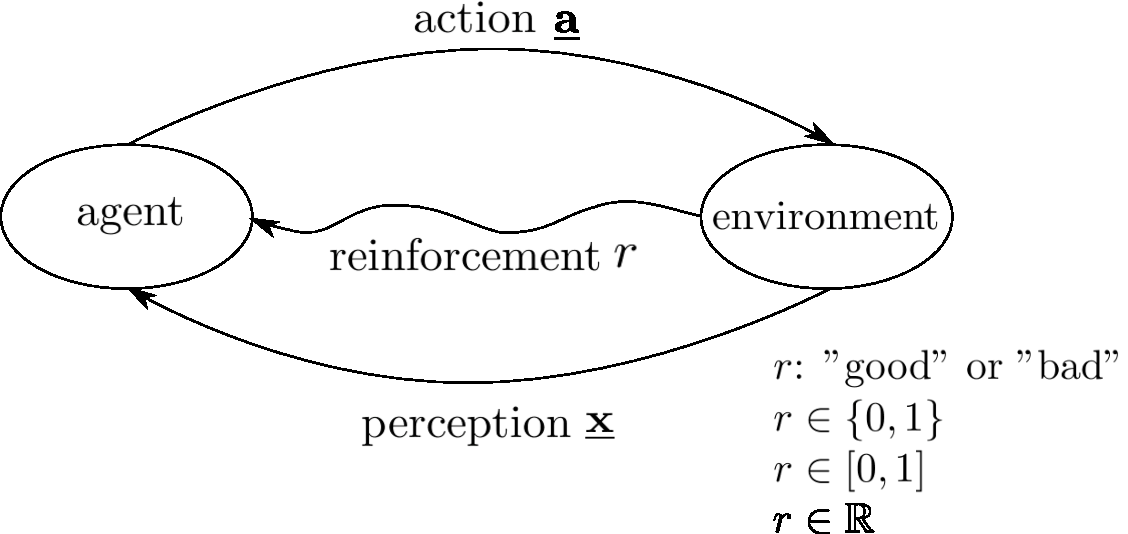
\includegraphics[width=10cm]{section4_fig1}
	\end{center}
\subsection{Reinforcement Learning -- Evaluation}
\subsubsection{Conditioning}
\paragraph{Classical conditioning}
	\begin{itemize}
				\item Ivan Pavlov (1849--1936)
				\vspace{2mm}
				\item 
\includegraphics[width=2mm]{neutral_stimulus}:
					conditioned stimulus (neutral)
				\vspace{2mm}
				\item 
\includegraphics[width=4mm]{rewarded_stimulus}:
					unconditioned stimulus (rewarding)
				\vspace{2mm}
				\item experience reinforces {\em involuntary response}
				\vspace{2mm}
				\item animal learns to {\em expect} reward
			\end{itemize} 
\begin{center}
		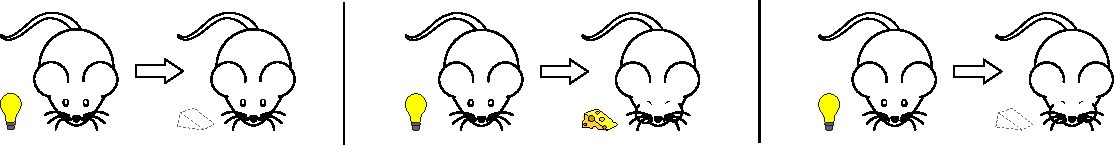
\includegraphics[width=12cm]{section4_fig2}
\end{center}
\paragraph{Operant conditioning}\mbox{}\\
\begin{minipage}{\textwidth}
		\begin{minipage}{7.75cm}
			\begin{itemize}
				\item B.F.~Skinner (1904--1990)
				\vspace{2mm}
				\item animal has to act voluntarily
				\vspace{2mm}
				\item actions are rewarded or punished
				\vspace{2mm}
				\item experience reinforces {\em voluntary behavior}
				\vspace{2mm}
				\item animal learns how to {\em achieve} reward
			\end{itemize} 
		\end{minipage}
		\hfill
		\begin{minipage}{4cm}
			\begin{center}
				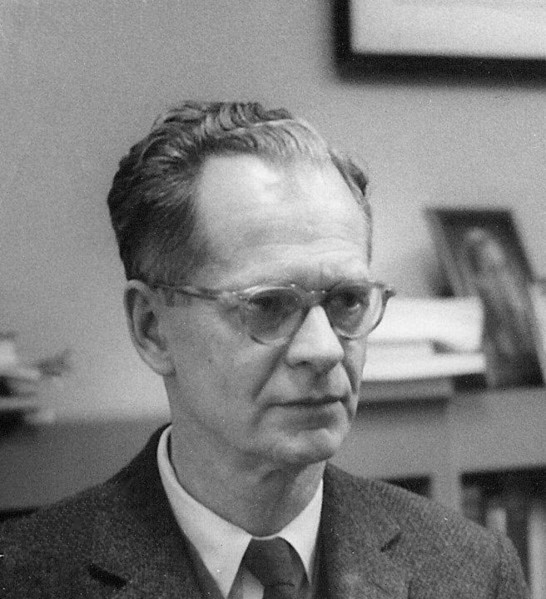
\includegraphics[width=3cm]{Skinner.jpg} \\
				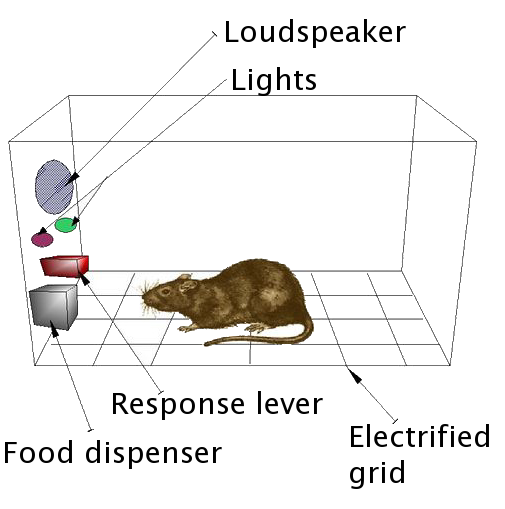
\includegraphics[width=4cm]{Skinner_box_scheme.png} 
			\end{center}
		\end{minipage}
	\end{minipage}
	
\paragraph{Future rewards}
	\begin{itemize}
		\item not all decisions are immediately rewarded
			\iitem{ decision in \textbf{state} $x_1$ is crucial, 
				but not rewarded}
		\vspace{2mm}
		\item some decisions require foresight 
			\iitem{future reward of decision in $x_1$ depends on 
				decisions in $x_2$ and $x_3$}
		\vspace{2mm}
		\item animal must {\em delay} the reinforcement of behavior
	\end{itemize}
	
	\vspace{2mm}
	\begin{center}
		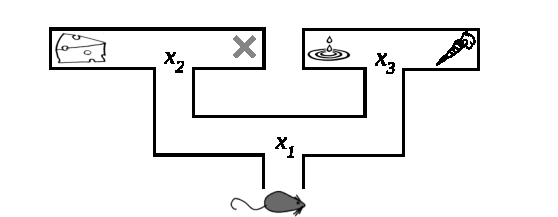
\includegraphics[width=6cm]{section4_fig3}
	\end{center}

\subsubsection{Markov Decision Processes}
\paragraph{Markov decision processes}\mbox{}\\
\begin{minipage}{\textwidth}
		\begin{minipage}{7.75cm}
			\begin{itemize}
				\item a set of \textbf{states} $\vec x \in \Set X$,
			\begin{itemize}
				\item e.g.~$\Set X := \{\vec x_1, \ldots, \vec x_S\} 
					\subset \{0,1\}^S$  \\with 1-out-of-$S$ encoding
			\end{itemize}
			\end{itemize} 
		\end{minipage}
		\hfill
		\begin{minipage}{4cm}
			\begin{center}
				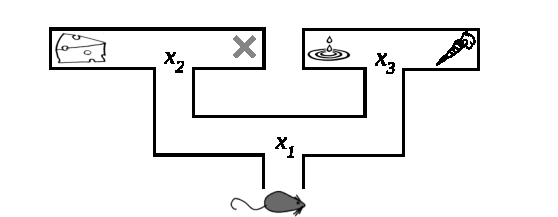
\includegraphics[width=5cm]{section4_fig3} \\
			\end{center}
		\end{minipage}
	\end{minipage}

\begin{minipage}{\textwidth}
		\begin{minipage}{7.75cm}
			\begin{itemize}
			\item a set of \textbf{actions} $\vec a \in \Set A$,
			\begin{itemize}
				\item e.g.~$\Set A := \{\vec a_1, \ldots, \vec a_A\} 
					\subset \{0,1\}^A$ \\ with 1-out-of-$A$ encoding
			\end{itemize}
			\end{itemize} 
		\end{minipage}
		\hfill
		\begin{minipage}{4cm}
			\begin{center}
				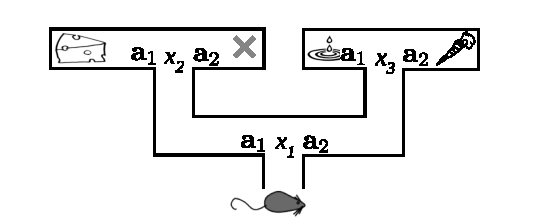
\includegraphics[width=5cm]{section4_fig4} \\
			\end{center}
		\end{minipage}
	\end{minipage}

\begin{minipage}{\textwidth}
		\begin{minipage}{7.75cm}
			\begin{itemize}
			\item a {\color{trans}\textbf{transition model} 
			$P(\vec x_j|\vec x_i, \vec a_k)$}
			\begin{itemize}
				\item probability to end up in $\vec x_j$ 
					after choosing $\vec a_k$ in $\vec x_i$
				\item stationary distribution (Markov property)
			\end{itemize}
			\end{itemize} 
		\end{minipage}
		\hfill
		\begin{minipage}{4cm}
			\begin{center}
				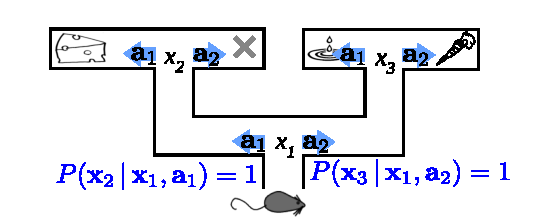
\includegraphics[width=5cm]{section4_fig5} \\
			\end{center}
		\end{minipage}
	\end{minipage}

\begin{minipage}{\textwidth}
		\begin{minipage}{7.75cm}
			\begin{itemize}
			\item a bounded {\color{reward}\textbf{reward function} 
			$r(\vec x_i, \vec a_k)$}
			\begin{itemize}
				\item denotes the {\em average immediate reward} 
					for choosing $\vec a_k$ in $\vec x_i$
				\item extension with randomized rewards possible
			\end{itemize}
			\end{itemize} 
		\end{minipage}
		\hfill
		\begin{minipage}{4cm}
			\begin{center}
				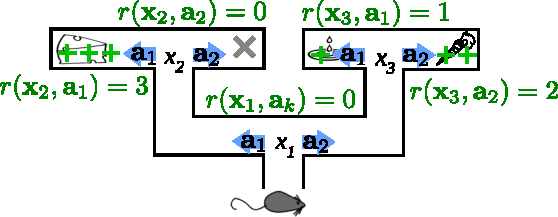
\includegraphics[width=5cm]{section4_fig6} \\
			\end{center}
		\end{minipage}
	\end{minipage}

\paragraph{Policy}
\begin{itemize}
		\item the agent's behavior is expressed by 
			a {\color{policy} \textbf{policy} $\pi(\vec a_k|\vec x_i)$}
			\begin{itemize}
				\item the probability that the agent 
					chooses $\vec a_k$ in $\vec x_i$
			\end{itemize}
	\end{itemize}
	\vspace{2mm}
	\begin{center}
		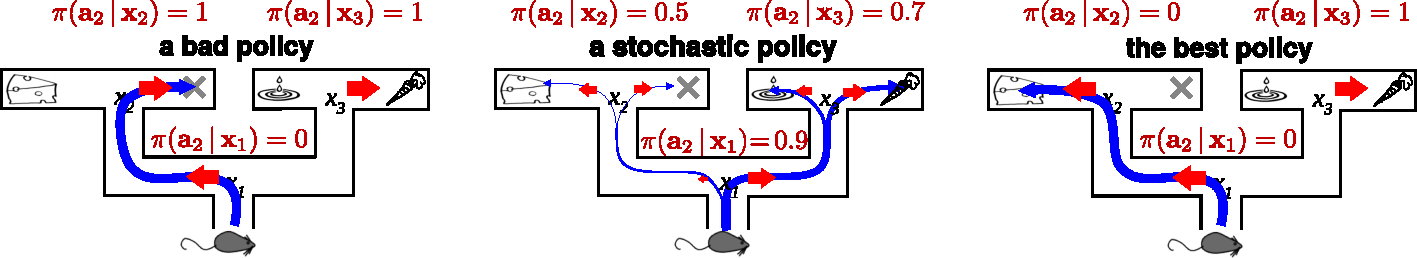
\includegraphics[width=\textwidth]{section4_fig7}
	\end{center}
	\iitem{the goal of RL is to find the ``\textbf{optimal policy}'' $\pi^*$}
	
\paragraph{Example: mountain car}\mbox{}\\
\begin{minipage}{12cm}
		\begin{minipage}{6.5cm}
			\begin{itemize}
				\item a car in a valley between mountains
					\iitem{$\Set X$: position and velocity}
				\vspace{2mm}
				\item agent drives the car
					\iitem{$\Set A$: forward, backward, nothing \\[-1.5mm]
						{\tiny (i.e., accelerate the car by $+a$, $-a$ and $0$)}}
				\vspace{2mm}
				\item dynamics are given by physics
					\iitem{{\color{trans}transition model $P$} simulated
					 \item gravitation but no friction}
				\vspace{2mm}
				\item{goal: reach right hilltop
					\iitem{{\color{reward}reward $r\kern-.5ex=\kern-.5ex0$}, 
							except {\color{reward}$r\kern-.5ex=\kern-.5ex1$} 
							at goal} }
				\vspace{2mm}
				\item but car is underpowered
					\iitem{{\color{policy}policy $\pi$} 
						must first pick up speed}
			\end{itemize}
		\end{minipage}
		\hfill
		\begin{minipage}{5.5cm}
			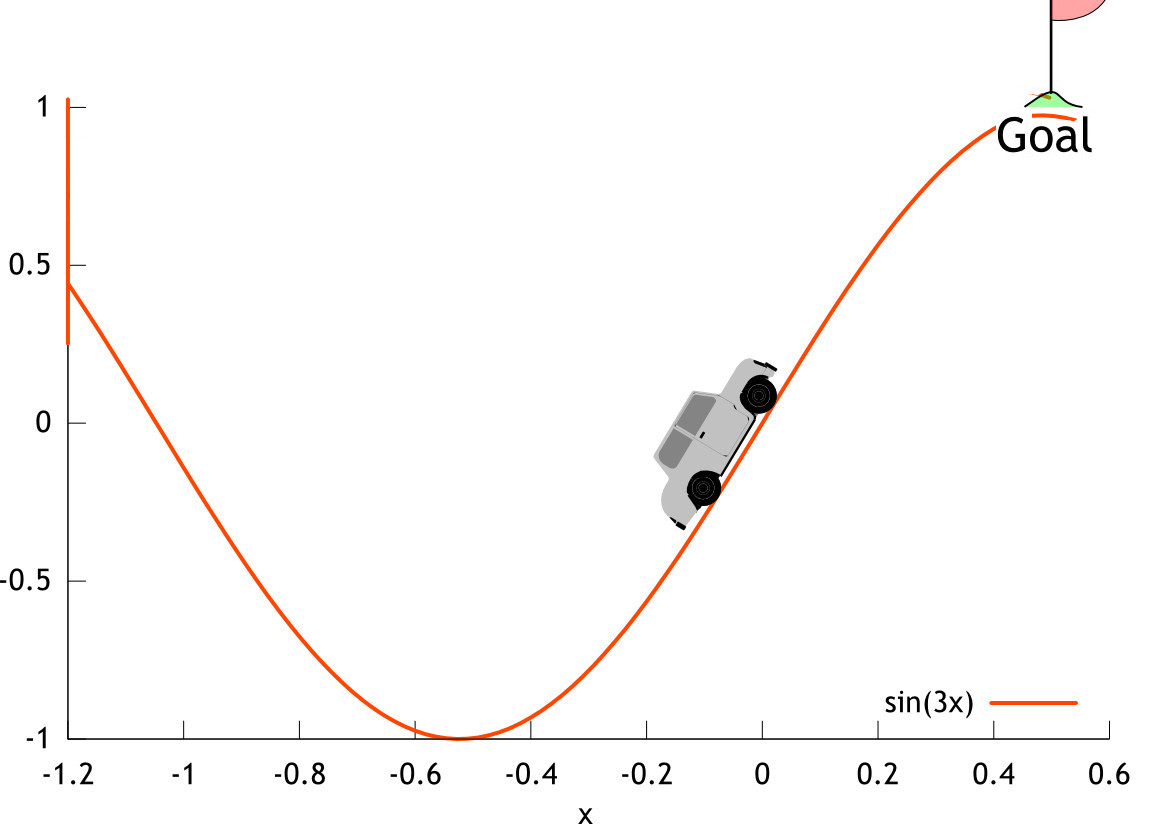
\includegraphics[width=\textwidth]{mountaincar2.jpg}
		\end{minipage}
	\end{minipage}
\paragraph{Markov chains}\mbox{}\\
\begin{minipage}{13cm}
		\begin{minipage}{7cm}
			\begin{itemize}
				\item a \textbf{Markov chain} of length $p$
					\vspace{2mm}
					\begin{itemize}
						\item  is a sequence  of states and actions
							$$
								\{\vec x^{(t)}, \vec a^{(t)}\}_{t=0}^{p} 
								\quad\subset\quad \Set X \times \Set A
							$$
						%\vspace{0mm}
						\item actions $\vec a^{(t)}$ 
							are drawn from {\color{policy}policy}: 
							$$
								\vec a^{(t)} \quad\sim\quad 
								{\color{policy}\pi(\cdot \,|\, \vec x^{(t)})}
							$$
						\item successive states $\vec x^{(t+1)}$
							are drawn from {\color{trans}transition model}:
							$$ 
								\vec x^{(t+1)} \quad\sim\quad 
								{\color{trans}P\big(\cdot|\, 
								\vec x^{(t)}, \vec a^{(t)}\big)}
							$$
					\end{itemize}
				\vspace{2mm}
				\item given an MDP, a Markov chain 
						depends on initial $\vec x^{(0)}$ 
						and {\color{policy}policy $\pi$}
			\end{itemize}
		\end{minipage}
		\begin{minipage}{5cm}
			\includegraphics[width=\textwidth]%
				{section4_fig8}
		\end{minipage}
	\end{minipage}

\paragraph{Markov chain distribution}\mbox{}\\
\begin{itemize}
		\item Markov chains are sets of random variables
			\iitem{ depend on initial state $\vec x^{(0)}$ 
				and {\color{policy}policy $\pi$} }
		\vspace{4mm}
		\item joint distribution of states in a Markov chain factorizes
			\vspace{-2mm}
			$$ 
				P(\vec x^{(0)}, \ldots, \vec x^{(p)})
				\;\;=\;\; P(\vec x^{(0)})
				\prod_{t=0}^{p-1} {\color{policy}\smallsum{k=1}{A}
					\pi(\vec a_k \,|\, \vec x^{(t)})} \,
					{\color{trans} P\big(\vec x^{(t+1)}|\, 
						\vec x^{(t)}, \vec a_k\big)}
			$$
	\end{itemize}
	\begin{center}
		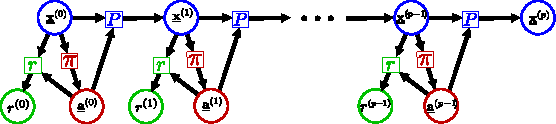
\includegraphics[width=11cm]{section4_fig9}
	\end{center}
% -----------------------------------------------------------------------------
% =============================================================================
\subsubsection{Policy Evaluation}
\definecolor{darkgreen}{rgb}{0,.5,0}
\definecolor{discount}{rgb}{.75,0,.75}
\definecolor{expect}{rgb}{0,.5,.5}
\definecolor{chain}{rgb}{.75,.5,0}

\paragraph{Value function}\mbox{}\\

\paragraph{Monte Carlo (MC) estimation of the value function}
\begin{figure}[h]
\centering
		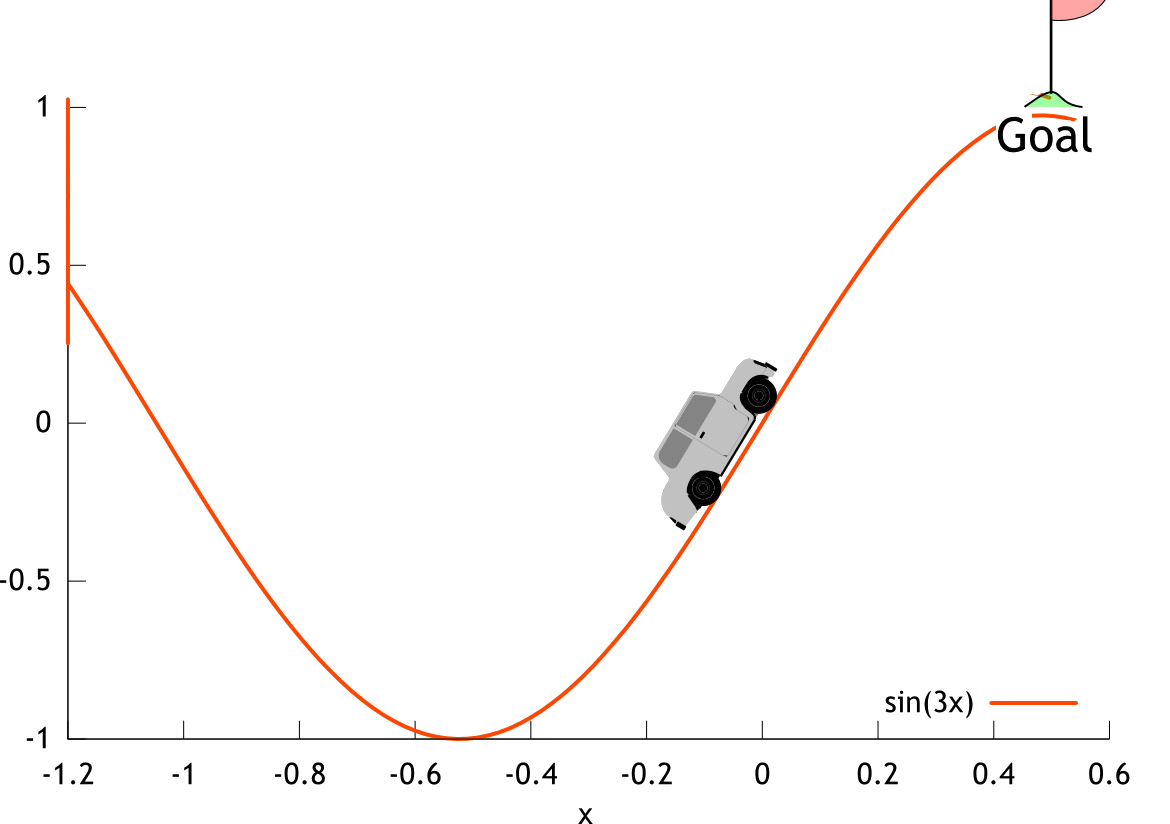
\includegraphics[width=4cm]{mountaincar2.png}
	\end{figure}

	\vspace{1mm}
	\begin{itemize}
		\item finite approximation of infinite Markov chains
			\vspace{.5mm}
			\begin{itemize}
				\item rewards weighted by $\gamma^H < \epsilon$ are neglected
				%\vspace{.5mm}
				%\item Markov chains of length $H$ are simulated
				\vspace{.5mm}
				\item value is the discounted reward averaged \\
					over $n$ Markov chains of length $H$
				\vspace{.5mm}
				\item $n$ must be sufficiently large
			\end{itemize}
		\vspace{2mm}
		\item requires simulator to draw $n$ chains 
			from the same initial state $\vec x^{(0)}$
		\vspace{2mm}
		\item every state must be evaluated often 
			$\leadsto$ not sample efficient
	\end{itemize}
	
	%\vspace{2mm}
	\begin{center}
		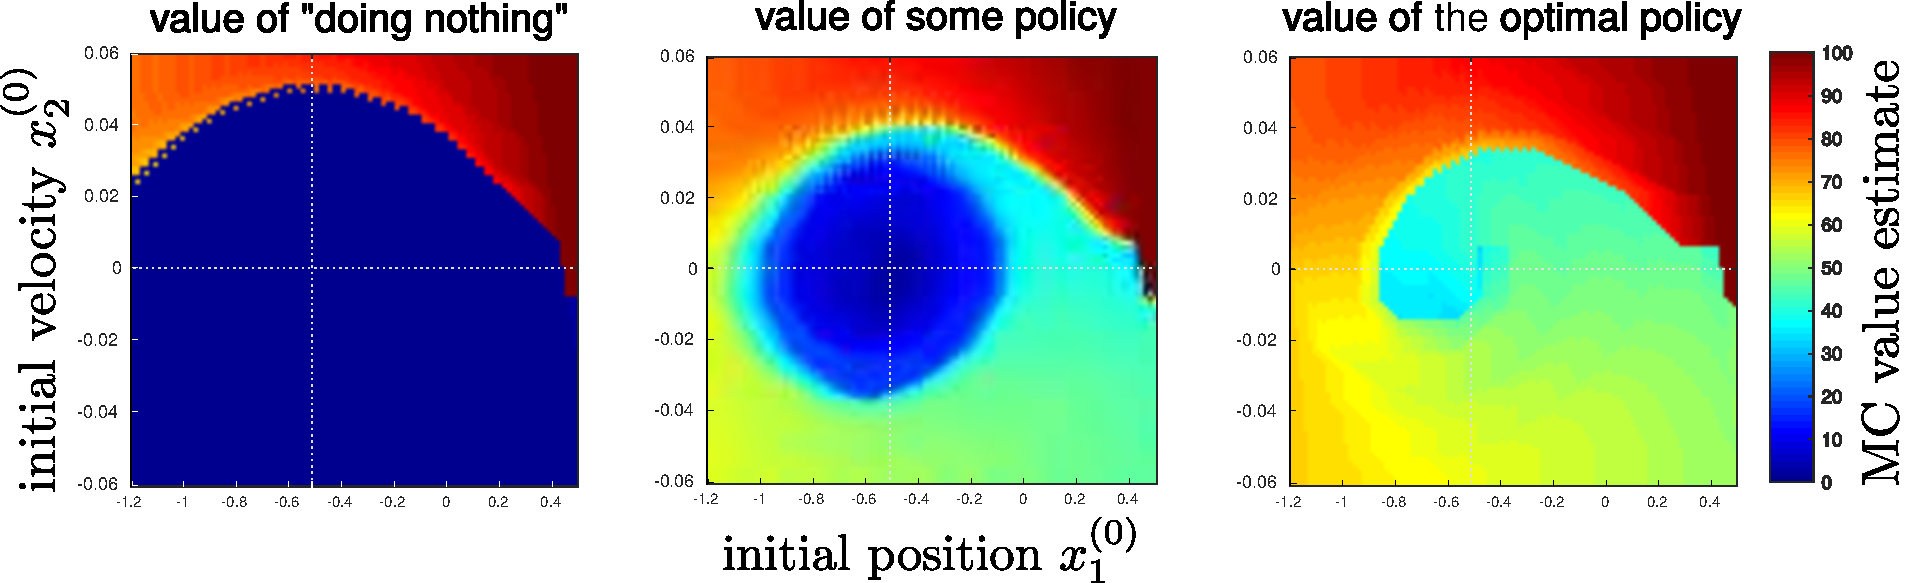
\includegraphics[width=12cm]{section4_fig10}
	\end{center}


\paragraph{The Bellman equation (1)}	
\begin{eqnarray*} %\hspace{-2mm}
		V^\pi(\vec x_i) 
		&=& \E\Bigg[ \sum_{t=0}^\infty \gamma^t \,
				{\color{reward}r(\vec x^{(t)}, \vec a^{(t)})} 
			\,\bigg| \begin{array}{c}
				\scriptstyle \vec x^{(0)} \;:=\;\; \vec x_i \hspace{11mm}\\[-1mm]
				\scriptstyle {\color{policy} \vec a^{(t)} \;\sim\;
					\pi(\cdot\,|\,\vec x^{(t)})} \;\;\;\\[-1mm]
				\scriptstyle {\color{trans}\vec x^{(t+1)} \;\sim\; 
					P(\cdot \,|\, \vec x^{(t)}, \vec a^{(t)}) }
			\end{array}\kern-1ex \Bigg] \\
		&=& \E\Big[ {\color{reward}r(\vec x_i, \vec a^{(0)})} \,\Big|\, 
				{\color{policy}\scriptstyle \vec a^{(0)} 
					\,\sim\, \pi(\cdot| \vec x_i)} 
			\Big] \\
		&& +\;\;  \E\Bigg[ 
				\sum_{t=1}^{\infty} \gamma^t \,
				{\color{reward}r(\vec x^{(t)}, \vec a^{(t)})} 
				\,\bigg| \begin{array}{c}
				\scriptstyle \vec x^{(0)} \;:=\;\; \vec x_i \hspace{11mm}\\[-1mm]
				\scriptstyle {\color{policy} \vec a^{(t)} \;\sim\;
					\pi(\cdot\,|\,\vec x^{(t)})} \;\;\;\\[-1mm]
				\scriptstyle {\color{trans}\vec x^{(t+1)} \;\sim\; 
					P(\cdot \,|\, \vec x^{(t)}, \vec a^{(t)}) }
			\end{array}\kern-1ex\Bigg] \\
		&=& \E\Big[ {\color{reward}r(\vec x_i, \vec a^{(0)})} \,\Big|\, 
				{\color{policy}\scriptstyle \vec a^{(0)} 
					\,\sim\, \pi(\cdot| \vec x_i)} 
			\Big] + \gamma \;\E\Big[ 
				V^\pi(\vec x^{(1)})
				\,\Big| \begin{array}{l}
					\scriptstyle {\color{policy} \vec a^{(0)} \;\sim\;
						\pi(\cdot\,|\,\vec x_i)} \\[-1mm]
					\scriptstyle {\color{trans} \vec x^{(1)} \;\sim\; 
						P(\cdot|\vec x_i, \vec a^{(0)})} 
			\end{array}\kern-1ex\Big] \\
		&=& {\color{policy} \sum_{k=1}^A \pi(\vec a_k \,|\, \vec x_i)}
			\Big( {\color{reward} r(\vec x_i, \vec a_k)}
			+ \gamma {\color{trans}\smallsum{j=1}{S} 
				P(\vec x_j \,|\, \vec x_i, \vec a_k)} \,
				V^\pi(\vec x_j) \Big) 
	\end{eqnarray*}
$\vec x_i \in \{0,1\}^S$: 1-out-of-$S$ coded state $i$

\paragraph{The Bellman equation (2)}
\begin{eqnarray*}
		V^\pi(\vec x_i) 
		&=&  
			{\color{policy} \sum_{k=1}^A \pi(\vec a_k \,|\, \vec x_i)}
			\Big( {\color{reward} r(\vec x_i, \vec a_k)}
			+ \gamma {\color{trans}\smallsum{j=1}{S} 
				P(\vec x_j \,|\, \vec x_i, \vec a_k)} \,
				V^\pi(\vec x_j) \Big) \\
		&=& 
			\underbrace{{\color{policy} \smallsum{k=1}A 
				\pi(\vec a_k \,|\, \vec x_i)} 
				{\color{reward} r(\vec x_i, \vec a_k)}
			}_{\kern-4ex\text{``controlled'' reward function }
					{\color{reward} r_i^\pi}\kern-4ex}
			\;+\; \gamma {\color{trans} \smallsum{j=1}{S}}
			\underbrace{
				{\color{policy} \smallsum{k=1}A 
				\pi(\vec a_k \,|\, \vec x_i)} 
				{\color{trans} P(\vec x_j \,|\, \vec x_i, \vec a_k)}
			}_{\text{``controlled'' transition model }
					{\color{trans} P^\pi_{ij}}}  V^\pi(\vec x_j) \\[4mm] 
		\vec v^\pi
		&=& {\color{reward}\vec r^\pi} 
			+ \gamma {\color{trans}\vec P^\pi} \vec v^\pi  \,,
		\quad \text{with}  \underbrace{ \left\{ \begin{array}{rcl} 
				{\color{reward}r^\pi_i} &\kern-1ex:=\kern-1ex& 
					{\color{policy} \smallsum{k=1}{A} 
					\pi(\vec a_k \,|\, \vec x_i)} \, 
					{\color{reward} r(\vec x_i, \vec a_k)} \\
				{\color{trans}P^\pi_{ij}} &\kern-1ex:=\kern-1ex& 
					{\color{policy}\smallsum{k=1}{A} 
					\pi(\vec a_k \,|\, \vec x_i)} \, 
					{\color{trans}P(\vec x_j | \vec x_i, \vec a_k)} \\
			\end{array} 
			\right.\kern-2ex}_{
				\text{``controlled'' models }
				{\color{reward}\vec r^\pi \in \R^S}
				\text{ and }{\color{trans}\vec P^\pi \in \R^{S \times S}}
			} \\[-12mm]
		&=:\kern-.5ex& \hat B^\pi[\vec v^\pi]
	\end{eqnarray*}
	\\
	$\vec x_i \in \{0,1\}^S$: 1-out-of-$S$ coded state $i$\\
	$\vec v^\pi \in \R^S$: vector containing all values $V^\pi$
	
\subsubsection{Model-based Approaches}
\paragraph{The analytic solution of the Bellman equation}\citep[see e.g.][for details]{Bertsekas07}\mbox{}\\
Bellman operator $\hat B^\pi$ for discrete state values:
	$$
				\hat B^\pi[\tilde{\vec v}] \quad=\quad
				{\color{reward}\vec r^\pi} 
				+ \gamma {\color{trans}\vec P^\pi} \tilde{\vec v} \,,
				\qquad\qquad \forall \tilde{\vec v} \in \R^S
	$$
\begin{itemize}
		\item Bellman operator $\hat B^\pi$ of {\color{policy}policy $\pi$}
			uses ``controlled'' models 
			\vspace{1mm}
			\iitem{of the reward function ${\color{reward}\vec r^\pi} \in \R^S$}
			\iitem{and transition model ${\color{trans}\vec P^\pi} 
					\in \R^{S \times S}$}
		\vspace{4mm}
		\item $\hat B^\pi$ has an analytic solution 
			of the value function $\vec v^\pi \in \R^S$
	\end{itemize}
	$$
	\vec v^\pi = {\color{reward}\vec r^\pi} 
		+ \gamma {\color{trans}\vec P^\pi} \vec v^\pi
	\;\;\leadsto\;\;
	\big(\vec I - \gamma {\color{trans}\vec P^\pi}\big) \vec v^\pi
		= {\color{reward}\vec r^\pi}
	\;\;\leadsto\;\;
	\vec v^\pi = \big(\vec I 
			- \gamma {\color{trans}\vec P^\pi}\big)^{-1}
		 {\color{reward}\vec r^\pi}
	$$
	\vspace{1mm}
	\begin{itemize}
		\item matrix $(\vec I - \gamma {\color{trans}\vec P^\pi}) 
			\in \R^{S \times S}$ is always invertible
			\vspace{1mm}
			\iitem{$|\lambda_k| \leq 1$ for all eigenvalues 
				$\lambda_k$ of transition matrices 
				${\color{trans}\vec P^\pi}$
			 \item discount factor $\gamma < 1$
			}
	\end{itemize}

\paragraph{Model-based value iteration}

\iitem{the value function $\vec v^\pi$ is the {\bf fixed-point} of 
			the Bellman operator $\hat B^\pi$}
	\vspace{1mm}
	$$	\vec v^\pi \quad=\quad 
		\hat B^\pi[\vec v^\pi] \quad=\quad
		{\color{reward}\vec r^\pi} 
		+ \gamma {\color{trans}\vec P^\pi} \vec v^\pi
	$$
	\iitem{{\bf value iteration}: repeated application of the Bellman operator}
	\vspace{3mm}
	$$
		\tilde{\vec v}^{\pi(t+1)} \quad=\quad {\color{reward}\vec r^\pi} 
				+ \gamma {\color{trans}\vec P^\pi} \tilde{\vec v}^{\pi(t)}
	$$
	\vspace{4mm}
	\iitem{is value iteration convergent, 
			i.e.~$\lim\limits_{t\to\infty} 
			\tilde{\vec v}^{\pi(t)} = \vec v^\pi$?}

\paragraph{Convergence of value iteration}\mbox{}\\

Contraction mapping (in supremum norm): \\
A function $\hat B : \R^S \to \R^S$ is called a 	
	{\em contraction mapping} 
		with Lipschitz constant $\lambda \kern-.5ex<\kern-.5ex 1$ if 
		$\max\limits_{j} 
		\big|(\hat B[\tilde{\vec v}] - \hat B[\tilde{\vec w}])_j \big| 
		\;\leq\; \lambda \max\limits_{j} \big|\tilde v_j - \tilde w_j \big|,
		\forall \tilde{\vec v}, \tilde{\vec w} \in \R^S$.
 
		\vspace{2mm}
		\iitem{application to the Bellman operator 
				$\hat B^\pi[\tilde{\vec v}] =
				{\color{reward}\vec r^\pi} 
				+ \gamma {\color{trans}\vec P^\pi} \tilde{\vec v}$}
		\begin{eqnarray*}
			\max_j \big| \hat B^\pi[\tilde{\vec v}]_j 
				- \hat B^\pi[\tilde{\vec w}]_j \big| 
			&=& \max_j
				\big| {\color{reward} r^\pi_j} 
					+ \gamma {\color{trans}(\vec P^\pi \tilde{\vec v})_j}
					- {\color{reward}r^\pi_j} 
					- \gamma {\color{trans}(\vec P^\pi \tilde{\vec w})_j} 
				\big| \\[-2mm]
			&\stackrel{\text{(i)}}{\leq}& 
				\max_j \gamma \, \big({\color{trans}\vec P^\pi} 
				|\tilde{\vec v} - \tilde{\vec w}|\big)_j 
			\quad\stackrel{\text{(ii)}}{\leq}\quad  
				\gamma \, \max_j |\tilde v_j - \tilde w_j|
		\end{eqnarray*}
		\vspace{2mm}
		\begin{eqnarray*}
			\text{(i)} \quad 
			 \Big|{\color{trans}\smallsum{i=1}{S} P^\pi_{ji}} \,x_i \Big|
			 	&\leq & 
				 {\color{trans} \smallsum{i=1}{S} P^\pi_{ji}} \, |x_i| \,,
				 \qquad\; \forall \vec x \in \R^S 
				 \hspace{1.2cm}\text{(Jensen's inequality)} \\[-1mm]
			\text{(ii)} \quad
			{\color{trans}\smallsum{i=1}{S} P^\pi_{ji}} \, |x_i|
				& \leq &
				{\color{trans} \smallsum{i=1}{S} P^\pi_{ji}}
					\max_{1\leq k\leq S} |x_k|
				\quad = \;\;\; \max_{1\leq k\leq S} |x_k| 
				\hspace{1.1cm}
				\text{(${\color{trans}\smallsum{i=1}{S} P^\pi_{ji} = 1}$)}
		\end{eqnarray*}

		\vspace{4mm}
		\begin{itemize}
			\item $\hat B^\pi$ is a contraction mapping 
				with Lipschitz constant $\gamma$
			\vspace{2mm}
			\begin{align} \tag{value iteration}
				\tilde{\vec v}^{\pi(t+1)} 
				\quad=\quad \hat B^\pi[\tilde{\vec v}^{\pi(t)}]
				\quad=\quad {\color{reward}\vec r^\pi} 
					+ \gamma {\color{trans}\vec P^\pi} \tilde{\vec v}^{\pi(t)}
			\end{align}
			\vspace{-2mm}
			\item $\max\limits_j \big|
				(\hat B^\pi[\vec v^{\pi(t)}])_j - v^\pi_j\big| 
				\leq \gamma \max\limits_j 
					\big|v^{\pi(t)}_j - v^\pi_j\big| $ 
				for {\em any} $\vec v^{\pi(t)} \in \R^S$
			\vspace{4mm}
			\item[$\Rightarrow$] value iteration converges in the limit
					to unique fix-point $\vec v^\pi$
				\vspace{1mm}
				\iitem{number of iterations until convergence 
					$\sim -\frac{1}{\log(\gamma)}$
				 \vspace{1mm}
				 \item analytic solution is faster for large $\gamma$
				}
		\end{itemize} 
		\vspace{4mm}


% =============================================================================
\subsubsection{Model-free Approaches: Online Value Estimation}
\paragraph{Inductive value estimation}
\iitem{agent must learn through interaction with the environment
		\vspace{1mm}
		\iitem{``controlled'' models ${\color{reward}\vec r^\pi}$ 
		and ${\color{trans}\vec P^\pi}$ are not available}}
	\vspace{4mm}
	$$
		V^\pi(\vec x_i) \quad=\quad 
			{\color{policy} \sum_{k=1}^A \pi(\vec a_k \,|\, \vec x_i)}
			\Big( {\color{reward} r(\vec x_i, \vec a_k)}
			+ \gamma {\color{trans}\smallsum{j=1}{S} 
				P(\vec x_j \,|\, \vec x_i, \vec a_k)} \,
				V^\pi(\vec x_j) \Big) 
	$$
	\vspace{4mm}
	\iitem{estimate value function {\em inductively} from one long Markov chain
		\vspace{1mm}
		\iitem{actions are drawn according to the {\color{policy}policy} 
		 	$ \vec a^{(t)} \sim {\color{policy}\pi(\cdot|\, \vec x^{(t)})}$
		 \vspace{1mm}
		 \item which lead to {\color{trans}transitions} 
		 		${\color{trans}\vec x^{(t+1)}
		 		\sim P(\cdot|\vec x^{(t)},\vec a^{(t)})}$
		 \vspace{1mm}
		 \item and yield {\color{reward} rewards 
		 		$r_t := r(\vec x^{(t)},\vec a^{(t)})$}
		 }
	}
\newcommand{\lr}{\eta}
\paragraph{Temporal difference (TD) learning}\citep[see][]{Sutton98}\mbox{}\\
\iitem{online estimation named after the difference in values (TD-error $\Delta V_t$)}
	$$
		\tilde V^{\pi}_{t+1}(\vec x^{(t)}) \quad = \quad 
		\tilde V^{\pi}_t(\vec x^{(t)}) \;+\;
		\lr \Big( \underbrace{{\color{reward}r_t} 
		+ \gamma \tilde V^{\pi}_t({\color{trans}\vec x^{(t+1)}}) 
		- \tilde V^{\pi}_t{(\vec x^{(t)})}}_{\text{TD-error }\Delta V_t} \Big) 
	$$
	
	\vspace{2mm}
	\iitem{TD learning performs value iteration {\em on average}
		\vspace{1mm}
		\iitem{for the average over all Markov chains 
			that pass $\vec x_i$ at time $t$ holds:
	}}
	$$
		\underbrace{\E\big[\tilde V^\pi_{t+1}(\vec x^{(t)})\big]
			}_{\tilde v_i^{\pi(t+1)}}
		\quad=\quad 
		(1 - \lr)\underbrace{\E\big[ \tilde V^\pi_t(\vec x^{(t)}) \big]
			}_{\tilde v_i^{\pi(t)}}
		\;+\; \lr \Big( \underbrace{\E[{\color{reward} r_t}]
		+ \gamma \E\big[\tilde V^\pi_t({\color{trans}\vec x^{(t+1)}})\big]
		}_{({\color{reward} \vec r^\pi} 
			+ \gamma {\color{trans} \vec P^\pi} \tilde{\vec v}^{\pi(t)})_i}\Big)
	$$
	
	\vspace{2mm}
	\iitem{{\em asynchronous online estimate} of 
			$\hat B^\pi[\tilde{\vec v}^{\pi(t)}] = {\color{reward}\vec r^\pi} 
			+ \gamma {\color{trans}\vec P^\pi} \tilde{\vec v}^{\pi(t)}$
		\vspace{1mm}
		\iitem{asynchronous update of one state at a time
		 \vspace{1mm}
		 \item estimates Bellman operator $\hat B^\pi$ by online average
		}
	}
\paragraph{Convergence of TD learning}
\iitem{{\bf example:} Markov chain running back and forth on 10 states
		\iitem{two randomly initialized 
			value functions ({\color{red}red}/{\color{blue}blue})
		 \item deterministic transitions with stochastic policy
		 \item rightmost state is rewarded, $\gamma=0.95$, $\lr=0.5$
		}
	 \vspace{1mm}
	 \item TD learning {\bf contracts} different initial values, 
		 	but does {\bf not converge} 
	}
	\begin{center}
		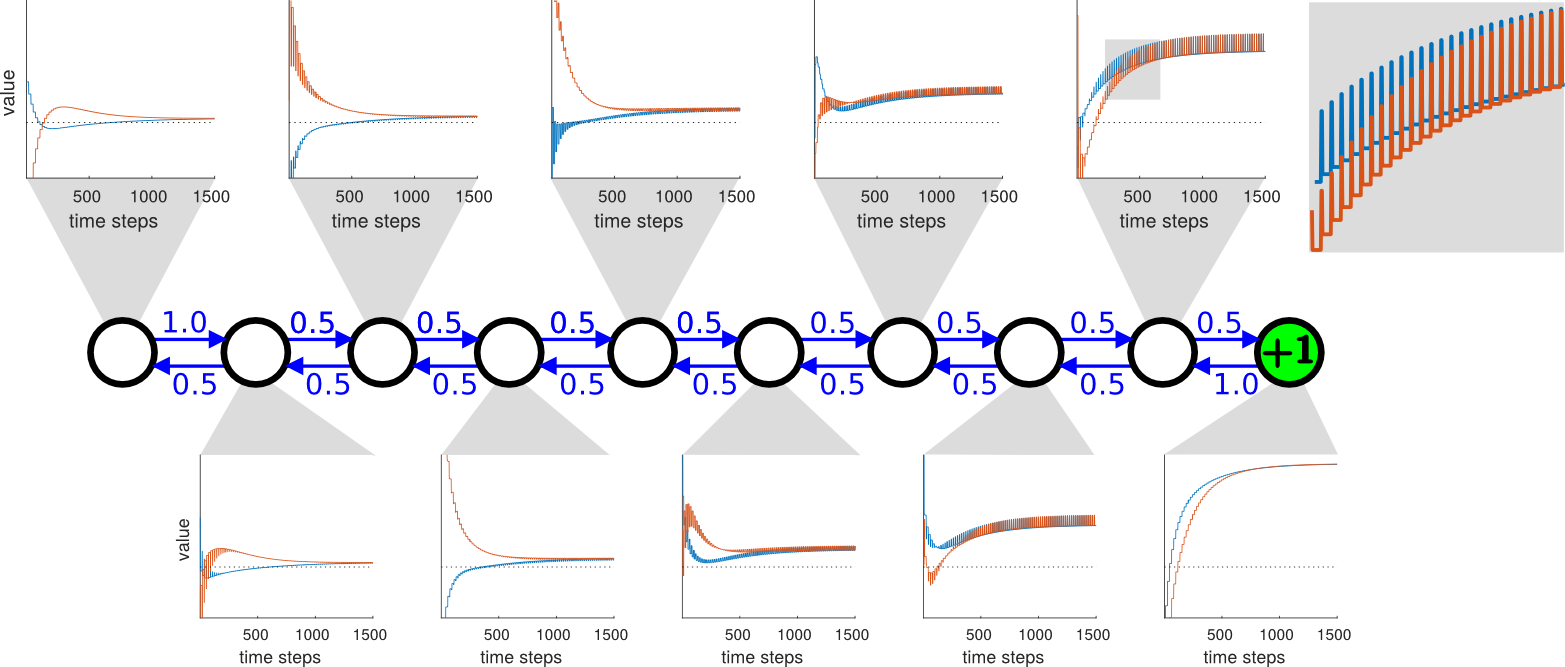
\includegraphics[width=\textwidth]{rl_chain_valuecontraction.png}
	\end{center}

\newcommand{\ssd}[1]{P_{\kern-.5ex\text{ss}}(\vec x_{{#1}})}
\paragraph{Requirements for contraction}\mbox{}\\
\begin{minipage}{12cm}
		\begin{minipage}{6.75cm}
			\begin{itemize}
				\item TD learning contracts 
					\vspace{1mm}
					\iitem{for an infinite Markov chain,
					 \vspace{1mm}
					 \item which visits {\em all} 
						states infinitely often}
				\vspace{5mm}
				\item no {\bf transient} transitions allowed
					 \vspace{1mm}
					 \iitem{transitions must be reversible
 					  \vspace{1mm}
					  \item ``you cannot learn from death''
					 }
			\end{itemize}
		\end{minipage}
		\hfill
		\begin{minipage}{5cm}
			\includegraphics[width=\textwidth]%
				{section4_fig11.pdf}
		\end{minipage}
	\end{minipage}
	
	\vspace{4mm}
	%\iitem{a state is called \textbf{transient} 
	%	if the Markov chain can never return to it
	%	\vspace{1mm}
		\iitem{\textbf{positive recurrence}:
			a non-zero probability to return in finite time}
	%}
\paragraph{Ergodic Markov chains}\mbox{}\\
Ergodicity: A Markov chain is {\bf ergodic} if it is
		{\bf positivly recurrent} 
		(non-zero probability to leave any state and 
		%a probability of 1 to 
		eventually return to it) and {\bf aperiodic} 
		(returns to the same state can occur at irregular times).
\begin{itemize}
		%\item infinite ergodic Markov chains visit every state infinitely often
		\item {\bf steady state distribution} 
			$\ssd{} > 0$ exists and visits all states $\vec x$ 
	\end{itemize}
%	$$
%		\ssd{j} \;\;=\;\; \sum_{i=1}^{S} \, \ssd{i} \;
%			\underbrace{{\color{policy}\smallsum{k=1}{A} 
%				\pi(\vec a_k \,|\, \vec x_i)} \;
%			{\color{trans}P(\vec x_j \,|\, \vec x_i, \vec a_k)} 
%				}_{{\color{trans}P_{ij}^\pi}}
%			\;\;=\;\; \sum_{i=1}^{S} \,\ssd{i}\, {\color{trans}P^\pi_{ij}}
%	$$
	\vspace{4mm}
	\begin{itemize}
		\item[$\Rightarrow$] TD learning is a contraction mapping 
			for {\em ergodic} Markov chains
	\end{itemize}

\paragraph{Influence of learning rate $\lr$}\mbox{}\\
\begin{minipage}{13cm} \hspace{-5mm}
		\begin{minipage}{6.75cm}
			{\footnotesize \begin{eqnarray*}
				\tilde V^{\pi}_{t+1}(\vec x^{(t)}) 
				&=& 
				\tilde V^{\pi}_t(\vec x^{(t)}) \;+\;
				\lr \, \Delta V_t \\
				\Delta V_t 
				&=&
				{\color{reward}r_t} 
				+ \gamma \tilde V^{\pi}_t({\color{trans}\vec x^{(t+1)}}) 
				- \tilde V^{\pi}_t{(\vec x^{(t)})}
			\end{eqnarray*}}
			\vspace{-4mm}
			\begin{itemize}
				\item stochastic transitions/rewards \\$\leadsto$ 
					$\tilde V^\pi_t$ may not converge
				\vspace{4mm}
				\item TD learning let $\tilde V^\pi_t$ fluctuate around \\ 
					 the true value function $V^\pi$ 
				\vspace{4mm}
				\item influence of the learning rate $\eta$
					\vspace{1mm}
					\begin{itemize}
						\item {\footnotesize large $\eta$: 
							fast learning, large variance}
						\vspace{1mm}
						\item {\footnotesize small $\eta$: 
							slow learning, small variance}
						\vspace{1mm}
						\item {\footnotesize decaying $\eta_t$ 
							are not practical as \\
							$\Delta V_t$ are (initially) not stationary}
					\end{itemize}
			\end{itemize}
		\end{minipage}
		\begin{minipage}{5.75cm}
			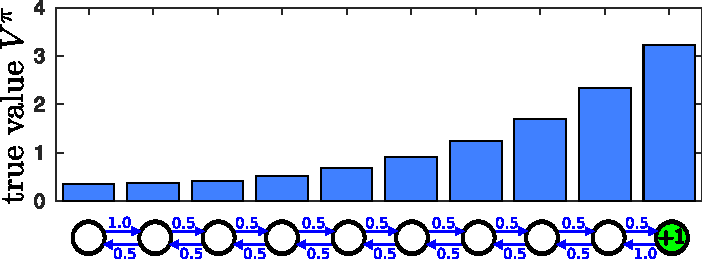
\includegraphics[width=\textwidth]{section4_fig12}
			
			\vspace{1mm}
			\footnotesize
			\begin{itemize}
				\item 10 states Markov chain 
				\item regular movement back and forth
				\item rightmost state rewarded, $\gamma = 0.95$
			\end{itemize}
			\vspace{1mm}			

			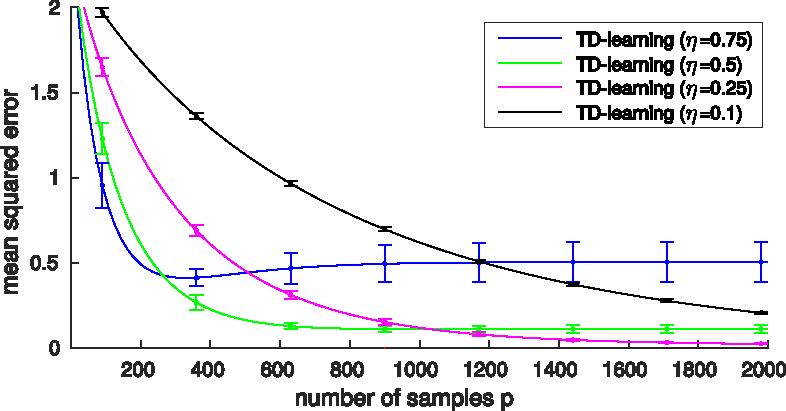
\includegraphics[width=\textwidth]{section4_fig13}
		\end{minipage}
	\end{minipage}


%%%==========================================================================
\subsubsection{Model-free Approaches: Eligibility Traces \& TD($\lambda$)}
\paragraph{Value propagation in TD learning}\mbox{}\\
\begin{minipage}{12.25cm}
		\begin{minipage}{6cm}
			{\footnotesize \begin{eqnarray*}
				\tilde V^{\pi}_{t+1}(\vec x^{(t)}) 
				&=& 
				\tilde V^{\pi}_t(\vec x^{(t)}) \;+\;
				\lr \, \Delta V_t \\
				\Delta V_t 
				&=&
				{\color{reward}r_t} 
				+ \gamma \tilde V^{\pi}_t({\color{trans}\vec x^{(t+1)}}) 
				- \tilde V^{\pi}_t{(\vec x^{(t)})}
			\end{eqnarray*}}
			\vspace{-4mm}
			\begin{itemize}
				\item TD learning propagates values one step into the past
					\iitem{many steps to convergence}
				\vspace{2mm}
				\item deterministic example:
					\begin{itemize}
						\item 10 states, 1 action 
						\item only forward transitions 
						\item reward in last state
						\item $\gamma = 0.9$; ${\color{red}\lr = 1}$ 
							or ${\color{darkgreen}\lr = 0.5}$
					\end{itemize}
				\vspace{2mm}
				\item value propagation requires
					\begin{itemize}
						\item exactly 10 rounds  
							(${\color{red}\lr = 1}$)
						\item roughly 26 rounds  
							(${\color{darkgreen}\lr = 0.5}$)
					\end{itemize}
			\end{itemize}
		\end{minipage}
		\hfill
		\begin{minipage}{5.8cm}
			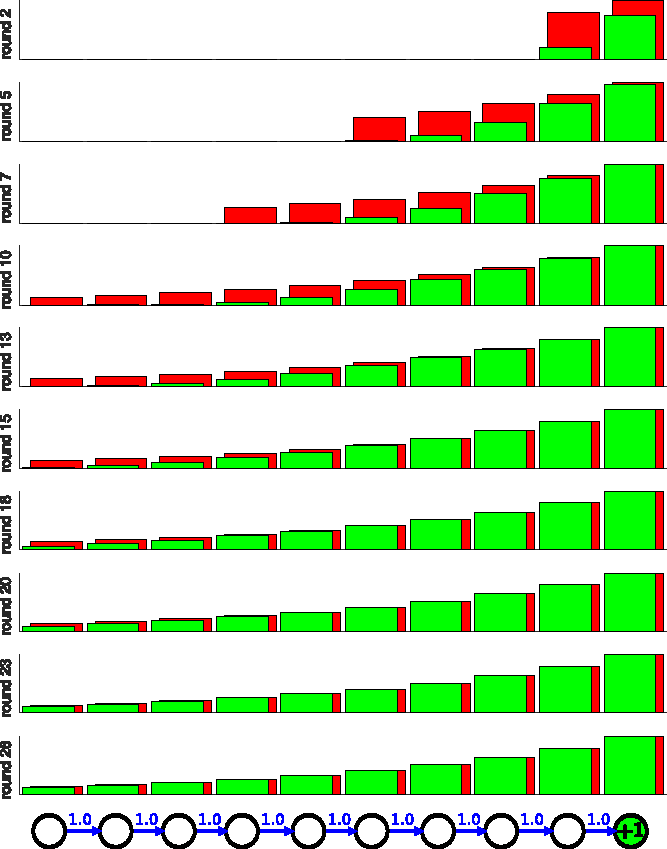
\includegraphics[width=\textwidth]{section4_fig14}
		\end{minipage}
	\end{minipage}
	
\paragraph{$n$-step temporal difference learning}\mbox{}\\
\iitem{accumulation of observed rewards}
	\begin{minipage}{13cm}
		\begin{minipage}{7.5cm}
			\begin{eqnarray*}
				R_t^{(1)} &=& {\color{reward}r_t} 
					+ \gamma \tilde V^\pi_t({\color{trans}\vec x^{(t+1)}})\\
				R_t^{(2)} &=& {\color{reward}r_t}  
					+ \gamma {\color{reward}r_{t+1}} 
					+ \gamma^2 \tilde V^\pi_t({\color{trans}\vec x^{(t+2)}}) \\
				&\vdots& \\
				R_t^{(n)} &=& \sum_{\tau=0}^{n-1} \gamma^\tau 
					{\color{reward}r_{t+\tau}} 
					+ \gamma^n \tilde V^\pi_t({\color{trans}\vec x^{(t+n)}})
			\end{eqnarray*}
		\end{minipage}
		\begin{minipage}{4.5cm}
			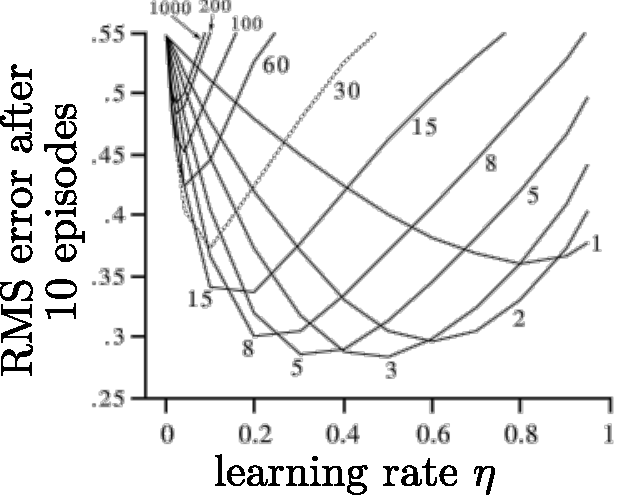
\includegraphics[width=\textwidth]{section4_fig15}\\[-8mm]
			\flushright
			\hfill{\tiny RMS averaged over 100 random-walks\\[-2mm] 
			on a 19-state chain, rewarded at one end}
		\end{minipage}
	\end{minipage}
	\vspace{-2mm}
	\iitem{online estimation similar to TD learning 
		\hfill {\footnotesize\citep{Sutton98}}}
		
	\vspace{-1mm}
	$$
		\tilde V^\pi_t(\vec x^{(t)}) \quad\leftarrow\quad 
		\tilde V^\pi_t(\vec x^{(t)}) \;+\; 
			\lr \Big( R_t^{(n)} - \tilde V^\pi_t(\vec x^{(t)}) \Big)
	$$

\paragraph{Discounted average}
$$
		\tilde V^\pi_{t+1}(\vec x^{(t)}) \quad\leftarrow\quad 
		\tilde V^\pi_t(\vec x^{(t)}) \;+\; 
			\lr \Big( R_t^{(n)} - \tilde V^\pi_t(\vec x^{(t)}) \Big)
	$$	
	\iitem{there is an optimal combination of $\eta$ and $n$, however,
	 \vspace{1mm}
	 \iitem{agent must memorize the last $n$ steps
	  \vspace{1mm}
	  \item values are updated with a delay of $n$ steps}
	}
	\vspace{4mm}
	\iitem{trick: consider a discounted average of $R^{(n)}_t$}
	$$
		R^\lambda_t \quad=\quad (1-\lambda) \,
		\sum_{k=0}^\infty \lambda^{k} \, R^{(k+1)}_t
	$$

\paragraph{Forward view}\mbox{}\\
	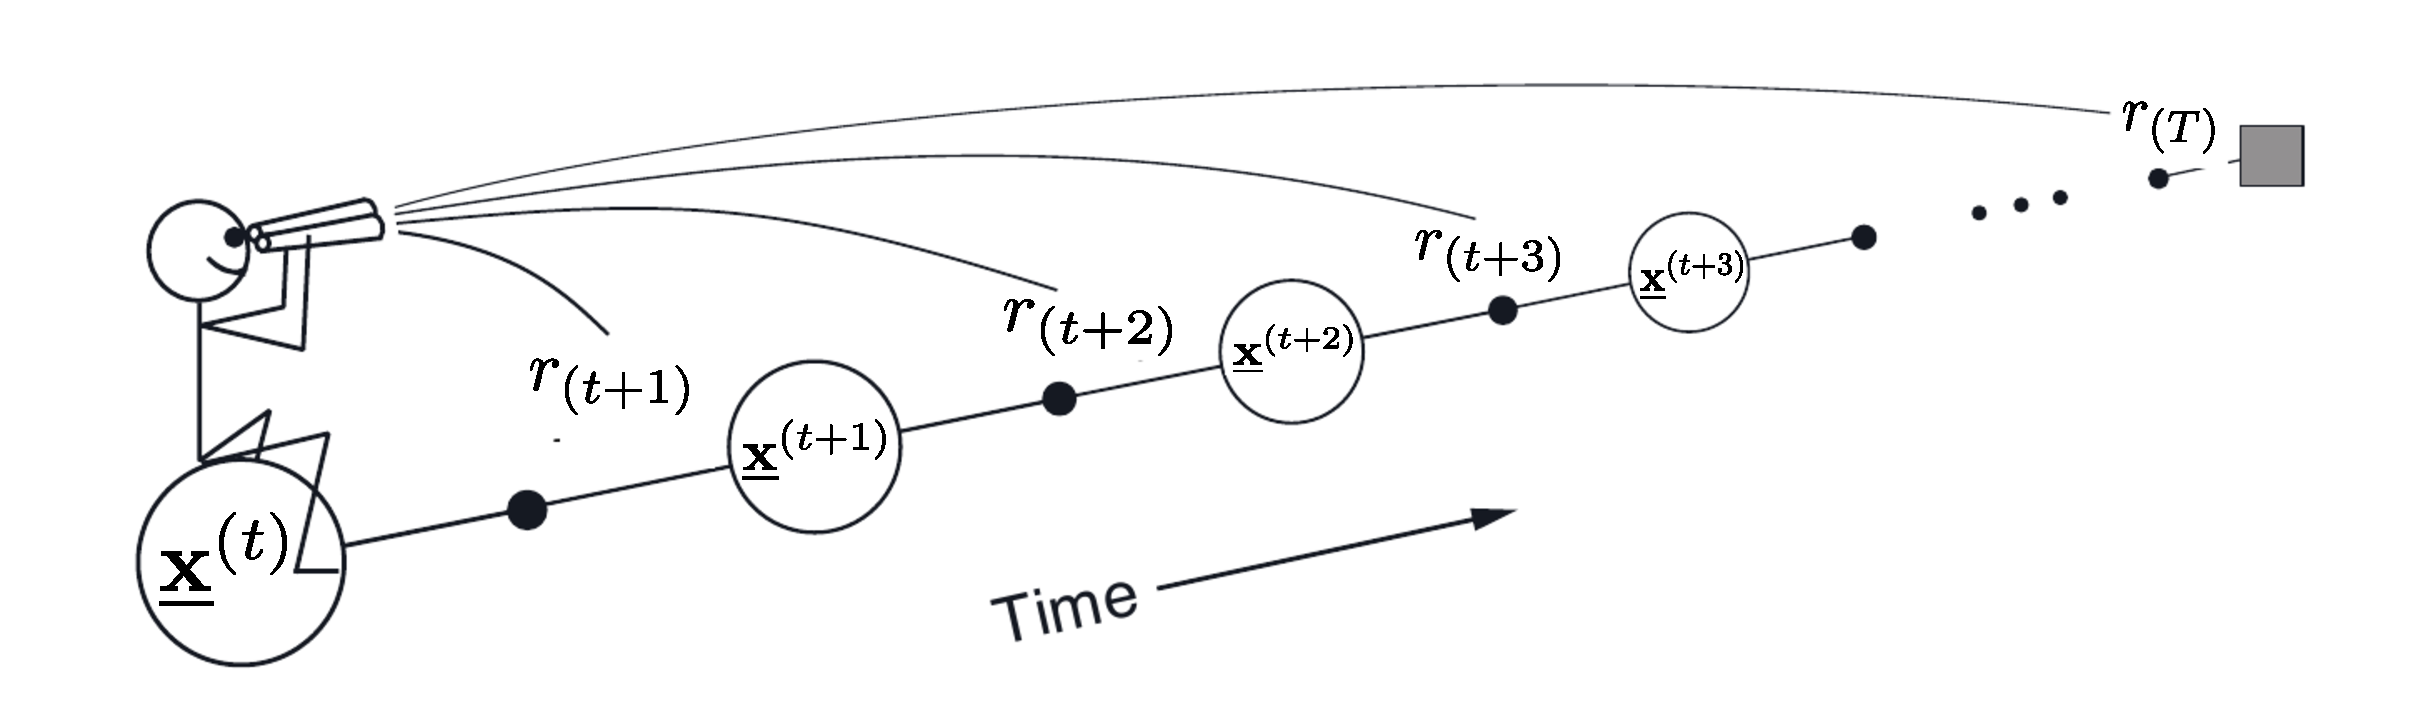
\includegraphics[width=\textwidth]{section4_fig16}
	
$$
	 \tilde V^{F}_{t+1}(\vec x^{(t)}) = \tilde V^{F}_t(\vec x^{(t)}) + \lr \Big( R_t^{\lambda} - \tilde V^{F}_t(\vec x^{(t)}) \Big)
$$	
$$
		R^\lambda_t \quad=\quad (1-\lambda) \,
		\sum_{k=0}^\infty \lambda^{k} \, R^{(k+1)}_t
$$

\definecolor{eligibility}{rgb}{.5,0,.5}
\paragraph{Eligibility traces \& TD($\lambda$)}
	\iitem{the {\bf eligibility trace} $\vec e^{(t)} \in \R^S$
		stores traces of past visits of state $\vec x_i$}
	$$
				e_i^{(t)} \quad=\quad 
				\sum_{k=0}^t (\gamma\lambda)^{t-k} \, \delta_{ik}  \,,
				\qquad \delta_{ik} = \vec x_i^\top \vec x^{(k)}
				\qquad \forall \vec x_i \in \Set X \,,
	$$
	\vspace{2mm}
	\iitem{The {\bf TD($\lambda$) method}:}
	\vspace{-6mm}
	\begin{eqnarray*}
		\tilde V^\pi_{t+1} (\vec x_i) 
		&=& \tilde V^\pi_t(\vec x_i) 
			\;+\; \lr \, {e_i}^{(t)} \,
			\big(\overbrace{
					{\color{reward}r_t} 
					+ \gamma \tilde V^\pi_t({\color{trans}\vec x^{(t+1)}})	
					- \tilde V^\pi_t(\vec x^{(t)})
			}^{\text{TD-error }\Delta V_t} \big)  \\
		\vec e^{(t+1)} &=&
			\gamma \, \lambda \, \vec e^{(t)} \;+\; \vec x^{(t+1)}
	\end{eqnarray*}
	
	\begin{minipage}{\textwidth}
		\begin{minipage}{5cm}
			\vspace{2mm}
			\begin{itemize}
				\item TD(0): TD learning
						as defined before
			\end{itemize}
			
			\vspace{1mm}
			\begin{flushright}
			{\tiny RMS averaged over 100 random-walks\\[-2mm]
			 on a 19-state chain, rewarded at one end}\\
			{\footnotesize \citep{Sutton98}}
			\end{flushright}
		\end{minipage}
		\hspace{10mm}
		\begin{minipage}{4cm} 
			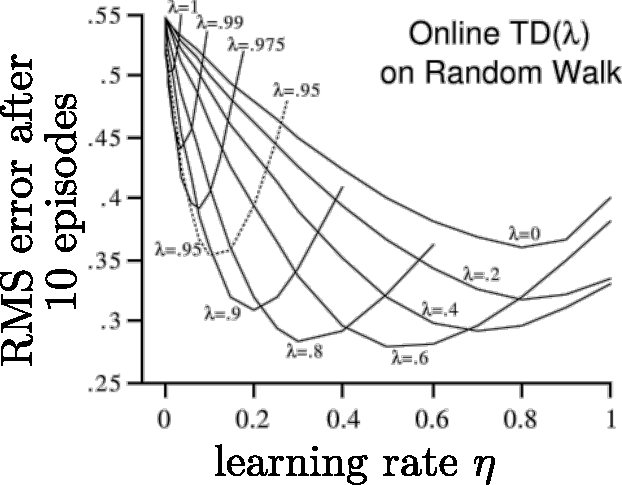
\includegraphics[width=\textwidth]{section4_fig17}
		\end{minipage}
		\hspace{1cm}
	\end{minipage}
	
\paragraph{Backward view}\mbox{}\\
	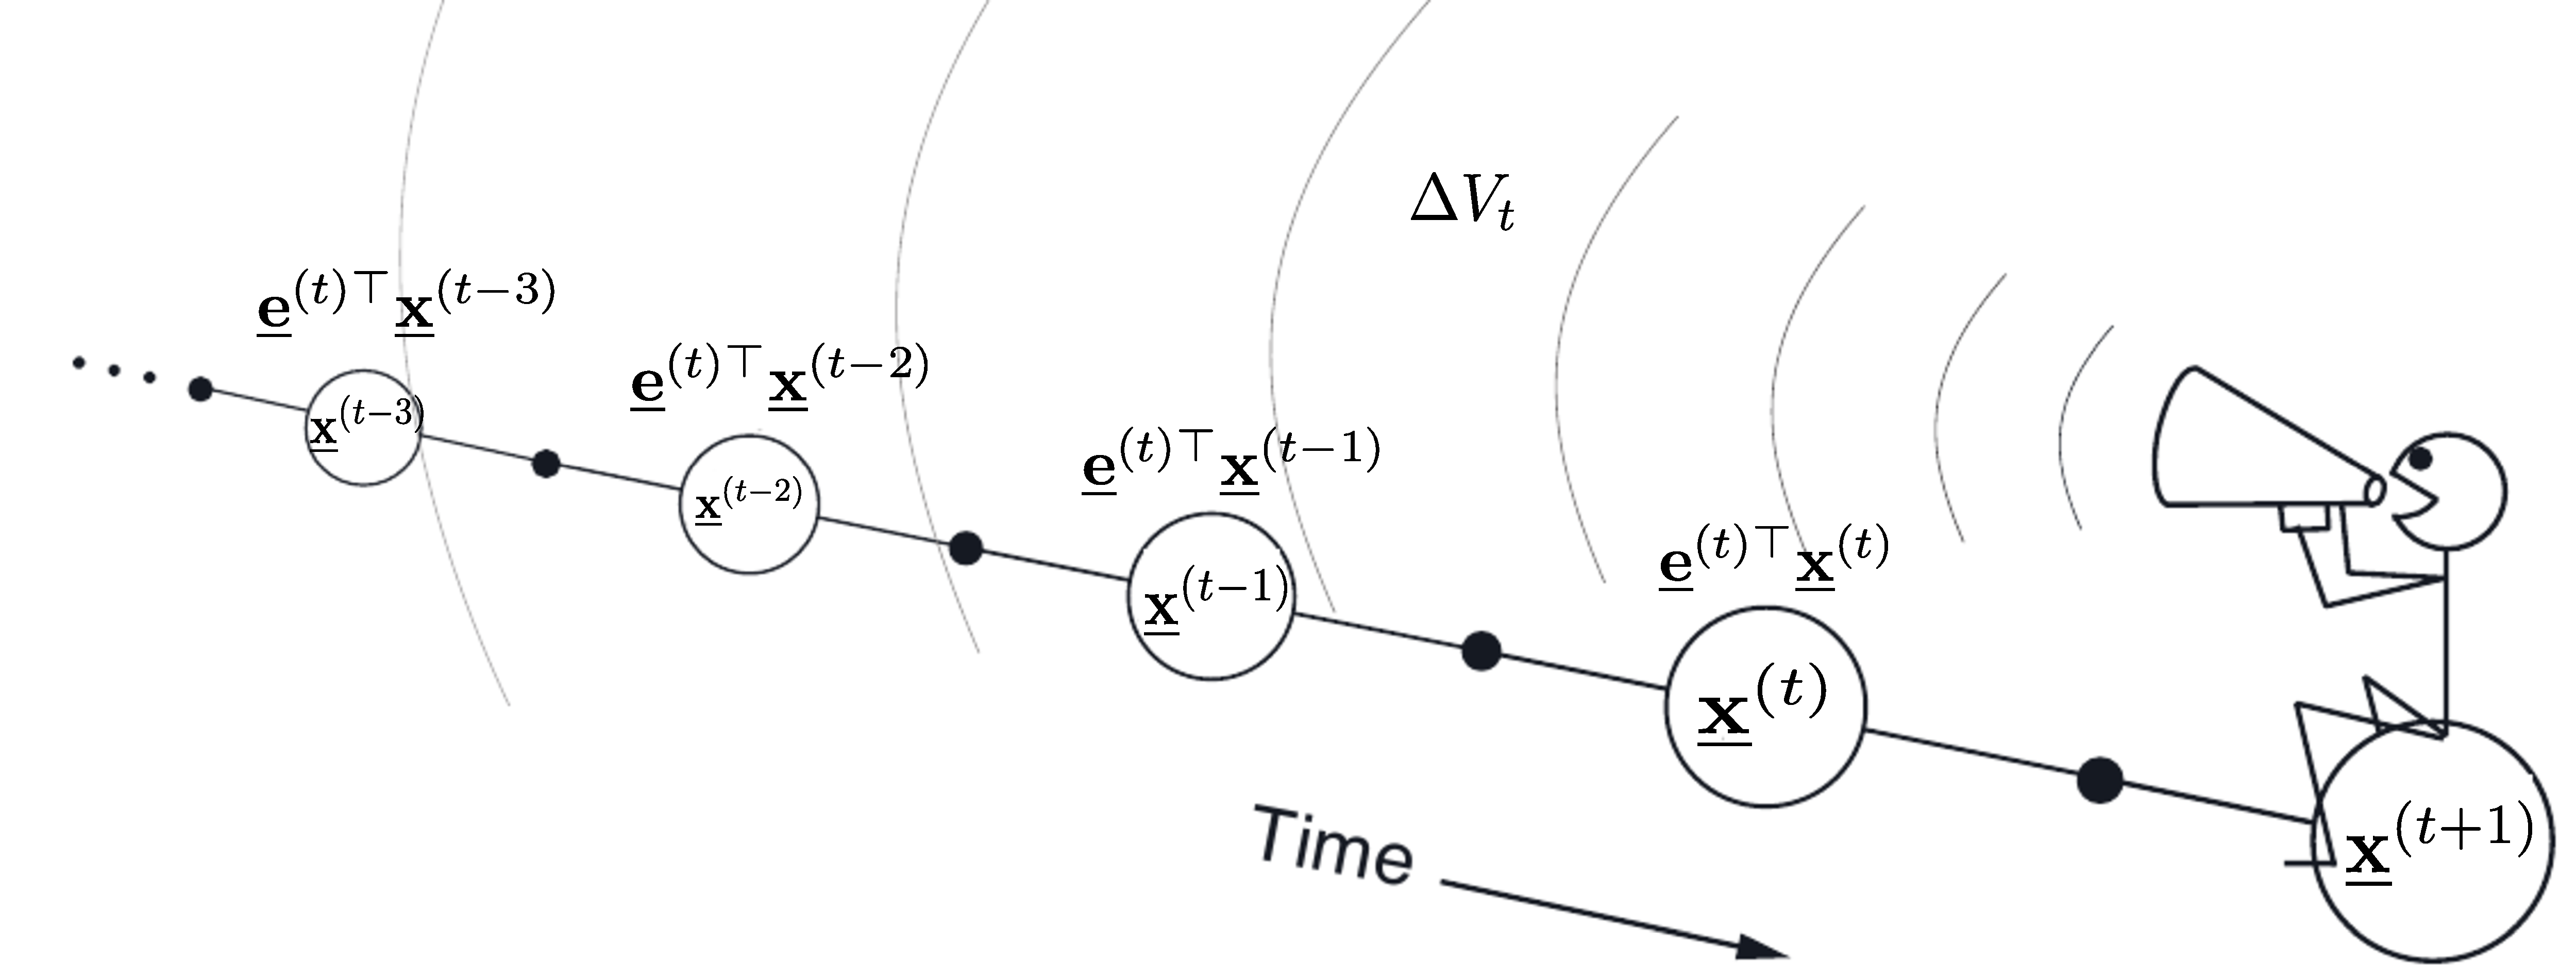
\includegraphics[width=\textwidth]{section4_fig18}
$$
		 \tilde V^{B}_{(t+1)}(\vec x_i) 
		 = \tilde V^{B}_{(t)}(\vec x_i)
		 	+\lr e_i^{(t)} \Delta V_t, \quad \Delta V_t 
		 = \big( r_t + \gamma \tilde V^{B}_t({\vec x^{(t+1)}})	
					- \tilde V^{B}_t(\vec x^{(t)})
			 \big)
$$
\vspace{-5mm}
$$
\vec e^{(t+1)} =\gamma \lambda \vec e^{(t)} + \vec x^{(t+1)}
$$
\vspace{-0.4cm}
\begin{itemize}
\item Both the forward and the backward view updates are \emph{equivalent}
\end{itemize}
\vspace{-0.2cm}


\paragraph{TD($\lambda$) derivation: the backwards view}
	\iitem{we use \quad$(1 - \lambda) \smallsum{i=0}{\infty} \lambda^i  = 1$ 
		\quad and \quad
		$\smallsum{i=0}{n} \, \smallsum{j=0}{i} A_{ij} 
		 = \smallsum{j=0}{n} \, \smallsum{i=j}{n} A_{ij}$}
	\iitem{The forward value at time $t$ is called $V^F_t$,
			the TD($\lambda$) value $V^B_t$}
	\iitem{the TD-error at time $t$ is $\Delta V_t 
		= r_t + \gamma V_t^{F/B}(\vec x^{(t+1)}) - V_t^{F/B}(\vec x^{(t)})$} 
	\hfill {\small ($F/B \rightarrow$  Forward or Backward view, whichever applies)}
	\begin{eqnarray*}
		V^B_T(\vec x_i) 
		&=& \smallsum{t=0}{T-1} \eta \; \Delta V_t \; e_i^{(t)} 
		\quad=\quad \eta \smallsum{t=0}{T-1}  \Delta V_t 
				\smallsum{k=0}{t} (\gamma\lambda)^{t-k} \, \delta_{ik} \\
		&=& \eta \smallsum{k=0}{T-1} \delta_{ik} 
			\smallsum{t=k}{T-1} (\gamma\lambda)^{t-k} \, \Delta V_t \\
		&=& \eta \smallsum{t=0}{T-1} \delta_{it} 
			\smallsum{k=t}{T-1} (\gamma\lambda)^{k-t} \, \Delta V_k
	\end{eqnarray*}

\paragraph{TD($\lambda$) derivation: the forwards view}
	\vspace{-4mm}
	\begin{eqnarray*}\hspace{-2mm}
		%\Delta V^F_t &:=& 
		R_t^\lambda - V_t^F(\vec x^{(t)}) \kern-2ex
		&=&\kern-2ex
		%\quad=\quad 
			(1-\lambda) \smallsum{k=0}{\infty} \lambda^k R_t^{(k+1)} 
			- V_t^F(\vec x^{(t)})\\
		&=&\kern-2ex 
			(1-\lambda) \smallsum{k=0}{\infty} \lambda^k 
			\Big( \smallsum{\tau=0}{k} \gamma^\tau r_{t+\tau} 
				+ \gamma^{k+1} V_t^F(\vec x^{(t+k+1)}) \Big)
			- V_t^F(\vec x^{(t)}) \\
		&=&\kern-2ex 
			(1-\lambda) \smallsum{\tau=0}{\infty} \, \smallsum{k=\tau}{\infty} 
			\lambda^k \gamma^\tau r_{t+\tau} 
			+ \gamma (1-\lambda) \smallsum{k=0}{\infty} \lambda^k \gamma^{k} 
				V_t^F(\vec x^{(t+k+1)}) 
			- V_t^F(\vec x^{(t)}) \\
		&=&\kern-2ex 
			\smallsum{\tau=0}{\infty} \gamma^\tau r_{t+\tau} \, \lambda^\tau
			\Big[(1-\lambda) \smallsum{k=0}{\infty} \lambda^k \Big]
			+ \gamma (1-\lambda) \smallsum{k=0}{\infty} (\gamma \lambda)^{k} 
				V_t^F(\vec x^{(t+k+1)}) 
			- V_t^F(\vec x^{(t)}) \\
		&=&\kern-2ex 
			\smallsum{k=0}{\infty} (\gamma\lambda)^k 
			\Big( r_{t+k} + \gamma V_t^F(\vec x^{(t+k+1)}) 
				- \gamma\lambda \, V_t^F(\vec x^{(t+k+1)}) \Big)
			- V_t^F(\vec x^{(t)}) \\
		&=&\kern-2ex 
			\smallsum{k=0}{\infty} (\gamma\lambda)^k 
			\Big( r_{t+k} + \gamma V_t^F(\vec x^{(t+k+1)}) 
				- V_t^F(\vec x^{(t+k)}) \Big) \\
		&\approx&\kern-2ex 
			\smallsum{k=0}{\infty} (\gamma\lambda)^k \, \Delta V_{t+k}
			\hspace{20mm}\text{(approximation is good for stationary $V_t^F$)} \\
		&\approx&\kern-2ex 
			\smallsum{k=t}{T-1} (\gamma\lambda)^{k-t} \, \Delta V_{k}
			\hspace{28mm}\text{(approximation is good for large  $T$)}
	\end{eqnarray*}

\paragraph{TD($\lambda$) derivation: both views}

	\iitem{the TD($\lambda$) value of state $\vec x_i$ at time $T$ is}
		$$
			V_T^B(\vec x_i) \quad=\quad 
			\eta \smallsum{t=0}{T-1} \delta_{it} 
			\smallsum{k=t}{T-1} (\gamma\lambda)^{k-t} \, \Delta V_k
		$$
	\iitem{the value of state $\vec x_i$ at time $T$ in the forward view is}
		\begin{eqnarray*}
			V_T^F(\vec x_i) 
			&=& \smallsum{t=0}{T-1} \eta \,\delta_{it} 
				\big(R_t^\lambda - V_t^F(\vec x^{(t)}) \big)
			\quad\approx\quad \eta \smallsum{t=0}{T-1} \delta_{it}
				 \smallsum{k=t}{T-1} (\gamma\lambda)^{k-t} \, \Delta V_{k}
		\end{eqnarray*}
	\iitem{in the limit of inifinite training samples the approximation is exact}
		\vspace{2mm}
		$$
			V_\infty^F(\vec x_i) \quad=\quad V_\infty^B(\vec x_i) 
		$$
		
\paragraph{Value propagation in TD learning}\mbox{}\\
	\begin{minipage}{12.25cm}
		\begin{minipage}{6cm}
			{\footnotesize \begin{eqnarray*}
				\tilde V^{\pi}_{t+1}(\vec x^{(t)}) 
				&=& 
				\tilde V^{\pi}_t(\vec x^{(t)}) \;+\;
				\lr \, \Delta V_t \\
				\Delta V_t 
				&=&
				{\color{reward}r_t} 
				+ \gamma \tilde V^{\pi}_t({\color{trans}\vec x^{(t+1)}}) 
				- \tilde V^{\pi}_t{(\vec x^{(t)})}
			\end{eqnarray*}}
			\vspace{-4mm}
			\begin{itemize}
				\item TD learning propagates values one step into the past
					\iitem{many steps to convergence}
				\vspace{2mm}
				\item deterministic example:
					\begin{itemize}
						\item 10 states, 1 action 
						\item only forward transitions 
						\item reward in last state
						\item $\gamma = 0.9$; ${\color{red}\lr = 1}$ 
							or ${\color{darkgreen}\lr = 0.5}$
					\end{itemize}
				\vspace{2mm}
				\item value propagation requires
					\begin{itemize}
						\item exactly 10 rounds  
							(${\color{red}\lr = 1}$)
						\item roughly 26 rounds  
							(${\color{darkgreen}\lr = 0.5}$)
					\end{itemize}
			\end{itemize}
		\end{minipage}
		\hfill
		\begin{minipage}{5.8cm}
			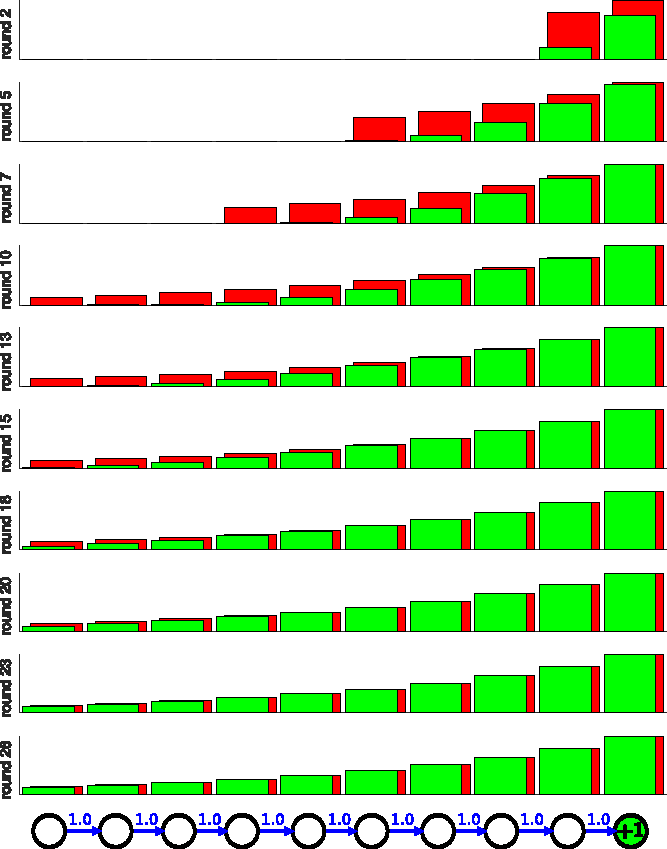
\includegraphics[width=\textwidth]{section4_fig19}
		\end{minipage}
	\end{minipage}
	
% =============================================================================
\subsubsection{Model-free approaches: Batch Value Estimation}
% -----------------------------------------------------------------------------
\paragraph{Reminder: the Bellman equation}
	\vspace{12mm}
	\begin{eqnarray*}
		V^\pi(\vec x_i) 
		&=& 
			\underbrace{{\color{policy} \smallsum{k=1}A 
				\pi(\vec a_k \,|\, \vec x_i)} 
				{\color{reward} r(\vec x_i, \vec a_k)}
			}_{\kern-4ex\text{``controlled'' reward function }
					{\color{reward} r_i^\pi}\kern-4ex}
			\;+\; \gamma {\color{trans} \smallsum{j=1}{S}}
			\underbrace{
				{\color{policy} \smallsum{k=1}A 
				\pi(\vec a_k \,|\, \vec x_i)} 
				{\color{trans} P(\vec x_j \,|\, \vec x_i, \vec a_k)}
			}_{\text{``controlled'' transition model }
					{\color{trans} P^\pi_{ij}}}  V^\pi(\vec x_j) \\[4mm] 
		\vec v^\pi
		&=& \hat B^\pi[\vec v^\pi] 
		\quad=\quad {\color{reward}\vec r^\pi} 
			+ \gamma {\color{trans}\vec P^\pi} \vec v^\pi 
	\end{eqnarray*}
	
	\vspace{4mm}
	{\footnotesize $\vec x_i \in \{0,1\}^S$: 1-out-of-$S$ coded state $i$\,,
		\hfill $\vec v^\pi \in \R^S$: vector containing all values $V^\pi$ \\
		${\color{reward} \vec r^\pi} \in \R^S$ ``controlled'' reward function\,,
		\hfill ${\color{trans}\vec P^\pi} \in \R^{S \times S}$
			``controlled'' transition model
	}	

\paragraph{Batch approximation of the Bellman operator (1)}\mbox{}\\
\begin{itemize}
		\item approximate $\tilde V_{t+1}^\pi \approx \hat B^\pi[\tilde V^\pi_t]$
			using samples from an\\
				{\color{trans}ergodic Markov chain} 
			$\{\vec x^{(t)}, \vec a^{(t)} \}_{t=0}^p$,
			{\color{policy}executing policy $\pi$} 
	\end{itemize}
	\vspace{-4mm}
	\begin{eqnarray*} \hspace{-9mm}
		\hat B^\pi[\tilde V^\pi_t](\vec x_i) &=&
		 	\underbrace{ {\color{policy} \sum_{k=1}^A 
		 		\pi(\vec a_k \,|\, \vec x_i)}
			\Big( {\color{reward}r(\vec x_i, \vec a_k)}
			+ \gamma \overbrace{
				{\color{trans}\smallsum{j=1}{S} 
					P(\vec x_j \,|\, \vec x_i, \vec a_k)} \,
				\tilde V^\pi_t(\vec x_j) \Big) }^{\text{average }
					\{\tilde V^\pi_t({\color{trans}\vec x^{(t+1)}}) 
						| \vec x^{(t)}=\vec x_i\}}
		}_{\text{approximate by averaging over } 
			\{\vec x^{(t)},\, \vec a^{(t)} \,|\, 
				\vec x^{(t)} = \vec x_i,\, 
				{\color{policy}\vec a^{(t)} \sim \pi} \} }\\[2mm]
				&\approx& \frac{1}{\underbrace{\textstyle\sum_{\tau=0}^{p-1} 
					\vec x_i^\top \vec x^{(\tau)}
					}_{\text{normalization}} 
				}\sum_{t=0}^{p-1} { 
					\underbrace{\vec x_i^\top \vec x^{(t)}
					}_{\text{selection}} 
				} %\only<3->{\quad\lr_t(\vec x_i)\quad}
			\Big( {\color{reward}r(\vec x^{(t)}, \vec a^{(t)})}
			+ \gamma \tilde V^\pi_t({\color{trans}\vec x^{(t+1)}}) \Big) 
	\end{eqnarray*}
	\iitem{$\vec x_i^\top \vec x^{(t)} = 1$ 
		only if $\vec x_i = \vec x^{(t)}$}
	\vspace{1mm}
	\iitem{$\sum_{\tau=0}^{p-1} \vec x_i^\top \vec x^{(\tau)}$
		counts how often $\vec x_i$ appears in Markov chain}

\paragraph{Batch approximation of the Bellman operator (2)}
	\begin{itemize}
		\item approximate $\tilde V_{t+1}^\pi \approx \hat B^\pi[\tilde V^\pi_t]$ 
			using samples from an\\
				{\color{trans}ergodic Markov chain} 
			$\{\vec x^{(t)}, \vec a^{(t)} \}_{t=0}^p$,
			{\color{policy}executing policy $\pi$} 
	\end{itemize}
	\begin{eqnarray*} \hspace{-3mm}
		\hat B^\pi[\tilde V^\pi](\vec x_i) 
%		&=&
%		 {\color{policy} \sum_{k=1}^A 
%		 		\pi(\vec a_k \,|\, \vec x_i)}
%			\Big( {\color{reward}r(\vec x_i, \vec a_k)}
%			+ \gamma {\color{trans}\smallsum{j=1}{S} 
%					P(\vec x_j \,|\, \vec x_i, \vec a_k)} \,
%				V(\vec x_j) \Big)  \\[2mm]
		&\approx& \frac{1}{\textstyle\sum_{\tau=0}^{p-1} 
					\vec x_i^\top \vec x^{(\tau)}}
			\sum_{t=0}^{p-1} \vec x_i^\top \vec x^{(t)}  
			\Big( {\color{reward}r(\vec x^{(t)}, \vec a^{(t)})}
			+ \gamma \tilde V^\pi({\color{trans}\vec x^{(t+1)}}) \Big) 	\\[2mm]
			&=& \kern-1ex\vec x_i^\top\kern-.5ex
				\Big( \underbrace{{\textstyle\smallsum{\tau=0}{p-1} 
					\vec x_i^\top \vec x^{(\tau)}}
					}_{C_{ii}} \Big)^{\kern-.5ex-1}
				\Big( \underbrace{\smallsum{t=0}{p-1} \vec x^{(t)} 
					{\color{reward}r(\vec x^{(t)}, \vec a^{(t)})}
					}_{{\color{reward}\vec b}}
				+ \gamma \, \underbrace{\smallsum{t=0}{p-1} \vec x^{(t)} 
					\tilde V^\pi({\color{trans}\vec x^{(t+1)}}) 
					}_{{\color{trans}\vec D^\pi} \tilde{\vec v}^\pi} \Big) \\[4mm]
		\hat B^\pi[\tilde{\vec v}^\pi]
		&\approx&
		\vec C^{-1} \big( {\color{reward}\vec b} + \gamma 
			{\color{trans} \vec D^\pi} \tilde{\vec v}^\pi \big)
	\end{eqnarray*}
	
	\vspace{4mm}
	\begin{minipage}{13cm} \hspace{-5mm}
		\begin{minipage}{4cm}
			\begin{center}	\scriptsize
				$\vec C = \smallsum{t=0}{p-1} \vec x^{(t)} (\vec x^{(t)})^\top
					\in\, \R^{S \times S}$\\ 
				diagonal normalization matrix 
			\end{center}
		\end{minipage}
		\begin{minipage}{4.4cm}
			\begin{center} \scriptsize
				${\color{trans}\vec D^\pi} = 
					\smallsum{t=0}{p-1} \vec x^{(t)} (\vec x^{(t+1)})^\top
					\in\, \R^{S \times S}$\\ 
				matrix of {\color{trans}transition} counts
			\end{center}
		\end{minipage}
		\begin{minipage}{4cm}
			\begin{center} \scriptsize
				${\color{reward}\vec b} = \smallsum{t=0}{p-1} \vec x^{(t)} 
					{\color{reward}r_{(\vec x^{(t)}, \vec a^{(t)})}}
					\,\in\, \R^{S}$\\ 
				vector of sum of {\color{reward}rewards}
			\end{center}
		\end{minipage}
	\end{minipage}

\paragraph{Example batch approximation}
	\iitem{the approximated Bellman operator:}
	$$ \hspace{-2cm} 
		\hat B^\pi[\tilde{\vec v}^\pi] \quad\approx\quad 
		\vec C^{-1} \big({\color{reward}\vec b} 
			+ \gamma {\color{trans}\vec D^\pi} \tilde{\vec v}^\pi \big) 
	$$
	
	\vspace{2mm}
	\begin{minipage}{12cm}
			\hspace{1cm}
			\begin{minipage}{3cm}
				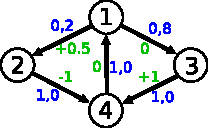
\includegraphics[height=2cm]{section4_fig20.pdf}
			\end{minipage}
			\begin{minipage}{7cm}
				\begin{itemize}
					\item example MDP with 4 states:
						\begin{itemize}
							\item example chain of length $p=30$
							\item {\color{trans} transition probabilities 
								$\vec P^\pi \approx \vec C^{-1} 
									{\color{trans}\vec D^\pi}$}
							\item {\color{reward} reward for transitions 
								\hspace{1.25mm} $\vec r^\pi \approx \vec C^{-1} 
								{\color{reward} \vec b}$}
						\end{itemize}
				\end{itemize}
			\end{minipage}
	\end{minipage}
	
	\vspace{2mm}
	$$
			\vec C = \left[ \begin{array}{cccc}
				10 & 0 & 0 & 0 \\
				0 & 3 & 0 & 0 \\
				0 & 0 & 7 & 0 \\
				0 & 0 & 0 & 10
			\end{array}\right] \,, 
			\qquad 
			{\color{blue}\vec D^\pi} = 
			\left[ \begin{array}{cccc}
				0 & \color{trans}3 & \color{trans}7 & 0 \\
				0 & 0 & 0 & \color{blue}3 \\
				0 & 0 & 0 & \color{blue}7 \\
				\color{blue}10 & 0 & 0 & 0
			\end{array}\right] \,,
			\qquad
			{\color{reward}\vec b} = 
			\left[ \begin{array}{c}
				\color{reward} 1.5 \\ 
				\color{reward} -3 \\ 
				\color{reward} +7 \\ 
				\color{reward} 0 
			\end{array} \right]
	$$
	{\footnotesize 
			\hspace{11mm} state visit counts 
			\hspace{26mm} {\color{trans}transition} counts
			\hspace{9mm} collected {\color{reward}rewards}
	}
	
	\vspace{6mm}
	\begin{minipage}{13cm} \hspace{-5mm}
		\begin{minipage}{4cm}
			\begin{center}	\scriptsize
				$\vec C = \smallsum{t=0}{p-1} \vec x^{(t)} (\vec x^{(t)})^\top
					\in\, \R^{S \times S}$
			\end{center}
		\end{minipage}
		\begin{minipage}{4.5cm}
			\begin{center} \scriptsize
				${\color{trans}\vec D^\pi} = 
					\smallsum{t=0}{p-1} \vec x^{(t)} (\vec x^{(t+1)})^\top
					\in\, \R^{S \times S}$
			\end{center}
		\end{minipage}
		\begin{minipage}{4cm}
			\begin{center} \scriptsize
				${\color{reward}\vec b} = \smallsum{t=0}{p-1} \vec x^{(t)} 
					{\color{reward}r_{(\vec x^{(t)}, \vec a^{(t)})}}
					\,\in\, \R^{S}$
			\end{center}
		\end{minipage}
	\end{minipage}

% -----------------------------------------------------------------------------
\paragraph{Solution to the approximated Bellman operator}
		

		\iitem{the approximated Bellman operator:}
	$$ \hspace{-2cm} 
		\hat B^\pi[\tilde{\vec v}^\pi] \quad\approx\quad 
		\vec C^{-1} \big({\color{reward}\vec b} 
			+ \gamma {\color{trans}\vec D^\pi} \tilde{\vec v}^\pi \big) 
	$$
	\begin{itemize}
		\item fixed-point $\vec v^* \approx \hat B^\pi[\vec v^*]$ 
				can be computed analytically
	\end{itemize}
		$$
			\vec v^* \;=\;  
			\big( \vec C - \gamma {\color{trans}\vec D^\pi} \big)^{-1}\, 
				{\color{reward}\vec b}\;=\; \big(\vec I - \gamma \underbrace{
						\vec C^{-1}{\color{trans}\vec {D}^\pi} 
						}_{\color{trans}\tilde{\vec P}^\pi}\big)^{-1} 
					\underbrace{\vec C^{-1} {\color{reward} \vec {b}}
						}_{\color{reward}\tilde{\vec r}^\pi}
				\;=\; 
				\big(\vec I - \gamma 
					{\color{trans}\vec {\tilde P}^\pi} \big)^{-1} 
				{\color{reward} \vec {\tilde r}^\pi}
		$$

			\begin{itemize}
				\item equivalent to empirically estimated model-based solution
			\end{itemize}
%			$$
%				{\color{trans}\vec{\tilde P}^\pi} 
%					\;\;=\;\; \vec C^{-1} {\color{trans}\vec D^\pi} \,, 
%				\qquad \text{and} \qquad
%				{\color{reward}\vec{\tilde r}^\pi} \;\;=\;\; \vec C^{-1} 
%				{\color{reward}\vec b}
%			$$
			{$$
				{\color{blue}\tilde{\vec P}^\pi} 
				\;=\; 
				\vec C^{-1} {\color{trans}\vec D^\pi} 
				{\;=\;
					\left[ \begin{array}{cccc}
						0 & \color{trans}.3 & \color{trans}.7 & 0 \\
						0 & 0 & 0 & \color{blue}1 \\
						0 & 0 & 0 & \color{blue}1 \\
						\color{blue}1 & 0 & 0 & 0
					\end{array}\right] 
				\,,}
				\qquad
				{\color{reward}\tilde{\vec r}} 
				\;=\; 
				\vec C^{-1} {\color{reward}\vec b} 
				{\;=\; 
					\left[ \begin{array}{c}
						\color{reward} .15 \\ 
						\color{reward} -1 \\ 
						\color{reward} +1 \\ 
						\color{reward} 0 
					\end{array} \right]
				}
			$$}
			\begin{itemize}
				\item in the limit convergence to $V^\pi$ 
					for ergodic Markov chains 
					\vspace{1mm}
					\iitem{${\color{trans}\tilde{\vec P}^\pi} 
						\to {\color{trans}\vec P^\pi}$
						and ${\color{reward}\tilde{\vec r}^\pi} 
						\to {\color{reward}\vec r^\pi}$
						if all states are visited infinitely often}
			\end{itemize}


\paragraph{Comparison of batch and online value estimation}\mbox{}\\
	\begin{minipage}{13cm}
		\begin{minipage}{6.4cm}
			\begin{itemize}
				\item reward propagation
					\begin{itemize}
						\item[TD(0):] {\footnotesize 
							one time step into the past}
						\item[TD($\lambda$):] {\footnotesize 
							all $\lambda$-discounted steps into the past}
						\item[batch:] {\footnotesize fix-point computation}
					\end{itemize}
				\vspace{4mm}
				\item different convergence behavior
					\begin{itemize}
						\item[TD(0):] fluctuates around $V^\pi$
						\item[TD($\lambda$):] fluctuates around $V^\pi$
						\item[batch:] converges to $V^\pi$
					\end{itemize}
				\vspace{4mm}
				\item computational complexities \\[-2mm]
					{\tiny (time and memory)}
					\begin{itemize}
						\item[TD(0):] $\Set O(p)$ and $\Set O(S)$
						\item[TD($\lambda$):] $\Set O(pS)$ and $\Set O(S)$
						\item[batch:] $\Set O(p+S^3)$ and $\Set O(S^2)$
					\end{itemize}
			\end{itemize}
			{\footnotesize $S$: number of states, \hfill $p$: number of samples}
		\end{minipage}
		\begin{minipage}{5.6cm}
			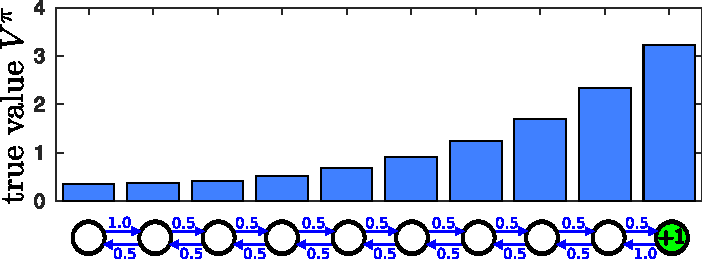
\includegraphics[width=\textwidth]{section4_fig21}
			
			\vspace{1mm}
			\footnotesize
			\begin{itemize}
				\item Markov chain back and forth
				\item only last state rewarded
				\item value estimated for $\gamma = 0.95$
			\end{itemize}
			\vspace{1mm}			

			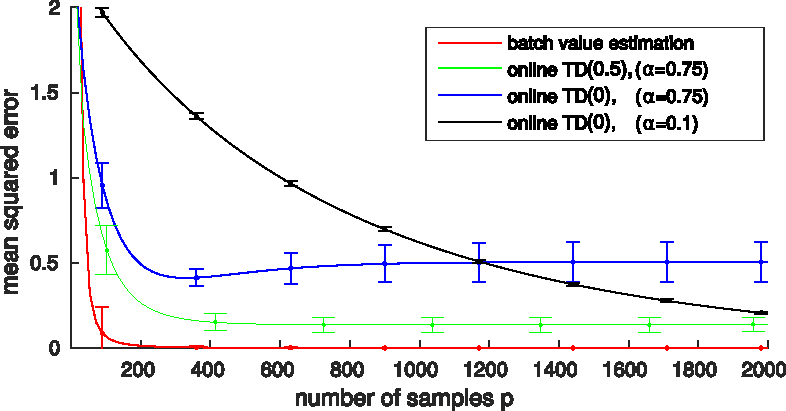
\includegraphics[width=\textwidth]{section4_fig22}
		\end{minipage}
	\end{minipage}
\paragraph{Neurological relevance of reinforcement learning}
			\begin{itemize}
				\item dopamine neurons encode TD-errors in many species
				\item model-based prediction errors 
						were found in human {\em pre-frontal cortex}
			\end{itemize}
		\slideref{Ex:Neurological relevance of reinforcement learning}

\subsection{Reinforcement Learning -- Improvement}
\subsubsection{Policy Improvement}
\paragraph{Valuation of state-action pairs: Q-values}\mbox{}\\
	\begin{itemize}
		\item{so far: agents learns where to {\em expect} rewards
		\vspace{4mm}
		\item now: agents learn how to {\em act} to maximize rewards}
		\vspace{4mm}
		\item {\bf Q-value} is the value of state $\vec x_i$ 
			{\bf after} choosing action $\vec a_k$
	\end{itemize}
	
	$$
		Q^\pi(\vec x_i, \vec a_k) \quad=\quad 
		\E\bigg[ \,
			\smallsum{t=0}\infty \, \gamma^t \,  
				{\color{reward}r(\vec x^{(t)}, \vec a^{(t)})}
			\, \bigg| \begin{array}{l}
				\scriptstyle \vec x^{(0)} =\, \vec x_i \,, \quad 
					\vec a^{(0)} =\, \vec a_k \\[-1mm]
				\scriptstyle {\color{trans} \vec x^{(t+1)} 
					\,\sim\, P(\cdot|\vec x^{(t)}, \vec a^{(t)})}\\[-1mm]
				\scriptstyle {\color{policy} \vec a^{(t+1)} 
				\,\sim\, \pi(\cdot|{\color{trans}\vec x^{(t+1)}})}
			\end{array}	
		\bigg]
	$$
Bellman equation for Q-values:\\
		\vspace{-4mm}	
		$$
			Q^\pi(\vec x_i, \vec a_k) \;\;=\;\; 
			{\color{reward} r(\vec x_i, \vec a_k)} \;+\; 
			\gamma {\color{trans} \sum_{j=1}^S 
				P(\vec x_j | \vec x_i, \vec a_k)} \;
				\underbrace{{\color{policy} \smallsum{l=1}{A} \, 
					\pi(\vec a_l | {\color{trans}\vec x_j})} \,
					Q^\pi({\color{trans}\vec x_j}, 
						{\color{policy}\vec a_l})
				}_{V^\pi({\color{trans}\vec x_j})}
		$$

\slideref{Ex: toy example}

\newcommand{\ind}[2]{\text{\raisebox{10pt}{\tiny%
	$\Big[\kern-2ex\begin{array}{c}%
	{#1}\\[-.5mm]{#2}\end{array}\kern-2ex\Big]$}}}
	
\paragraph{Q-value estimation}\mbox{}\\
\begin{eqnarray*} 
		V^\pi(\vec x_i) &=&
			\overbrace{
				{\color{policy}\smallsum{k=1}{A} \pi(\vec a_k|\vec x_i)} \, 
				{\color{reward}r(\vec x_i, \vec a_k)}
			}^{{\color{reward}r^\pi(\vec x_i)}}
			\;+\; \gamma {\color{trans} \sum_{j=1}^{S}}
				\overbrace{{\color{policy}\smallsum{k=1}{A} 
						\pi(\vec a_k|\vec x_i)} 
					{\color{trans}P(\vec x_j|\vec x_i, \vec a_k)}
				}^{{\color{trans}P^\pi(\vec x_j|\vec x_i)}}
				V^\pi(\vec x_j) \\ 
	\hspace{-2.5mm}
		Q^\pi(\vec x_i, \vec a_k)
		&=& {\color{reward}r(\vec x_i, \vec a_k)}
			\;+\; \gamma {\color{trans}\sum_{j=1}^{S}} 
			{\color{policy}\sum_{l=1}^{A}} \,\underbrace{
			{\color{policy}\pi(\vec a_l|\vec x_j)} \,
			{\color{trans}P(\vec x_j | \vec x_i, \vec a_k)}
			}_{{\color{trans}P'^\pi(\vec x_j,\vec a_l| \vec x_i,\vec a_k)}} 
			Q^\pi(\vec x_j, \vec a_l)
	\end{eqnarray*}
\begin{itemize}
		\item ${\color{trans}P'^\pi}$ is a transition model
			in the space of states and actions
			\vspace{-2mm}
			$$
				{\color{trans}\smallsum{j=1}{S} \smallsum{l=1}{A} \;
					P'^\pi(\vec x_j,\vec a_l| \vec x,\vec a)}
				\quad=\quad 1 \,, \qquad \forall \vec x \in \Set X, \quad 
				\forall \vec a \in \Set A
			$$
		\item {\bf Q-values are value functions} of state-action pairs
			\vspace{1mm}
			\begin{itemize}
				\item with reward function ${\color{reward}r}$ 
					and transition model ${\color{trans}P'^\pi}$
				\vspace{1mm}
				\item all techniques for value estimation apply to Q-values		
				\vspace{1mm}
				\item much larger space $\leadsto$ requires more samples to estimate
			\end{itemize}
	\end{itemize}
\paragraph{SARSA}\mbox{}\\
\begin{itemize}
		\item inductive TD(0) learning for Q-values using TD-errors
			\vspace{1mm}
			\iitem{with \quad 
				${\color{trans}\vec x^{(t+1)} \sim 
					P(\cdot| \vec x^{(t)}, \vec a^{(t)})}$ 
				\quad and \quad ${\color{policy}\vec a^{(t+1)} 
					\sim \pi(\cdot | \vec x^{(t+1)})}$}
			\vspace{2mm}
			$$
				\Delta Q_t \quad=\quad {\color{reward}r_t} 
				\;+\; \gamma \, Q({\color{trans}\vec x^{(t+1)}}, 
					{\color{policy}\vec a^{(t+1)}}) 
				\;-\; Q(\vec x^{(t)}, \vec a^{(t)})
			$$
		\vspace{0mm}
		\item {\bf on-policy}: SARSA estimates the Q-values $Q^\pi$ 
			of sampling policy $\pi$ 
			\vspace{1mm}
			\iitem{named after the type of  training data: \\
				State$_t$-Action$_t$-{\color{reward}Reward$_t$}%
					-{\color{trans}State$_{t+1}$}%
					-{\color{policy}Action$_{t+1}$}}
		\vspace{4mm}
		\item a SARSA($\lambda$) variant with eligibility traces exists
	\end{itemize}
	\vspace{2mm}
SARSA algorithm for Q-value estimation:\\
		\For{$t \in \{0,\ldots,p-1\}$}{
			$Q_{(\vec x^{(t)},\vec a^{(t)})} \quad \leftarrow \quad
			Q_{(\vec x^{(t)},\vec a^{(t)})} \;+\; \lr \, 
				\Big(\underbrace{{\color{reward}r_t} + \gamma \, 
				  Q_{({\color{trans}\vec x^{(t+1)}}, 
				  	{\color{policy}\vec a^{(t+1)}})} 
				- Q_{(\vec x^{(t)}, \vec a^{(t)})}
			}_{\Delta Q_t} \Big)$ \\[-5mm]
		}

\paragraph{Off-policy value estimation}
	\begin{itemize}
		\item  {\color{policy}sampling policy} 
			affect SARSA updates through 
			${\color{policy}\vec a^{(t+1)} \sim \pi(\cdot|\vec x^{(t+1)})}$
			$$ \hspace{-21mm}
				\Delta Q_t \quad=\quad {\color{reward}r_t} 
				\;+\; \gamma \, Q({\color{trans}\vec x^{(t+1)}}, 
					{\color{policy}\vec a^{(t+1)}}) 
				\;-\; Q(\vec x^{(t)}, \vec a^{(t)})
			$$
		\vspace{0mm}
		\item why not estimate Q-values of a {\em different} 
			{\color{policy}policy $\pi'$} ({\bf off-policy}\footnote{
				Note that the concepts underlying TD($\lambda$) 
				cannot be applied to off-policy learning.
			})?
			$$
				\Delta Q'_t \quad=\quad {\color{reward}r_t} 
				\;+\; \gamma \, {\color{policy}\smallsum{k=1}{A}
					\pi'(\vec a_k \,|\, {\color{trans}\vec x^{(t+1)}})} \,
					Q({\color{trans}\vec x^{(t+1)}}, {\color{policy}\vec a_k}) 
				\;-\; Q(\vec x^{(t)}, \vec a^{(t)})
			$$
		\vspace{0mm}
		\item contracts for an ergodic Markov chain:
			$\lim\limits_{p\to\infty} \E\Big[
				\smallsum{t=0}{p} \Delta Q'_t 
			\Big]= Q^{\pi'}$
		\vspace{4mm}
		\item Markov chain $\{x_t,a_t,r_t\}_{t=1}^{p}$ 
		used for training can be reused when $\pi'$ changes!
	\end{itemize}
\paragraph{Optimal policy}
	\begin{itemize}
		\item the optimal policy $\pi^*$ should maximize
			value function $V^{\pi^*}$
		\vspace{4mm}
		\item maximizing values:
			\vspace{-2mm}
			\begin{eqnarray*}\hspace{-8mm}
				\max_{{\color{policy}\pi^*}} V^{\pi^*}(\vec x_i) 
				&=& \max_{{\color{policy}\pi^*}} 
					{\color{policy} \smallsum{k=1}{A} 
					\pi^*(\vec a_k|\vec x_i)} \, 
					Q^{\pi^*}(\vec x_i, \vec a_k) \\
				&=& {\color{policy}\max_{1 \leq k \leq A}} 
					Q^{\pi^*}(\vec x_i, {\color{policy}\vec a_k})
			\end{eqnarray*}
		\item $\pi^*$ chooses the action $\vec a_k$ with 
			the largest associated Q-value
		\vspace{2mm}
	\end{itemize}
	
{\bf Greedy policy} $\pi'$ on a Q-value function $Q^{\pi}$:\\
			$$
				\pi'(\vec a_k \,|\, \vec x_i) 
				\quad=\quad \left\{ \begin{array}{cl}
					1 &,\; \text{if} \; k = \argmax\limits_{1 \leq l \leq A} 
						Q^{\pi}(\vec x_i, \vec a_l) \\
					0 &,\; \text{otherwise}
				\end{array} \right.
			$$			
\paragraph{Policy iteration}
	\begin{itemize}
		\item any policy $\pi_i$ is {\em improved} by
			the greedy policy $\pi_{i+1}$ of Q-value $Q^{\pi_{i}}$:
			\vspace{1mm}	
			$$
				Q^{\pi_{i+1}}(\vec x_i, \vec a_k) 
					\quad\geq\quad Q^{\pi_{i}}(\vec x_i, \vec a_k)
			$$
		%\vspace{4mm}
		%\item alternating value estimation and policy improvement 
	\end{itemize}
	\vspace{4mm}
Policy iteration (PI):\\
		initialize first policy $\pi_{0}$ randomly\\
		\While{Q-values not converged}{
			estimate 
				%(with any algorithm) Q-value function 
				$\tilde Q^{\pi_i} :\approx Q^{\pi_i}$ of policy $\pi_i$ \\
			choose $\pi_{i+1}$ to be the greedy policy on $\tilde Q^{\pi_i}$
		} 
		
		\vspace{-4mm}
		{\footnotesize\hfill\citep[see]%
		[for convergence with estimated Q-values]{Bertsekas07}}

\paragraph{On-line policy improvement: Q-learning}
	{\small $$\hspace{-2mm}
			\tilde Q^*(\vec x^{(t)}, \vec a^{(t)})
			\;\; \leftarrow \;\;
			\tilde Q^*(\vec x^{(t)}, \vec a^{(t)})
			\;+\; \lr \Big( \underbrace{
				{\color{reward}r_t} + \gamma 
				\overbrace{
					{\color{policy} \max_{1 \leq k\leq A}}
					\tilde Q^*({\color{trans}\vec x^{(t+1)}}, 
						{\color{policy}\vec a_k})
				}^{\text{\kern-2exgreedy policy improvement\kern-2ex}}
				- \, \tilde Q^*(\vec x^{(t)}, \vec a^{(t)})	
				}_{\text{TD-error}\;\Delta Q_t }\Big)
	$$}
	\begin{itemize}
		\item Q-learning estimates the Q-value $Q^{\pi^*}$ of 
			the {\color{policy}optimal policy $\pi^*$}
		\vspace{4mm}
		\item Q-learning is a contraction mapping for {\em any} ergodic Markov chain
			\begin{center}
				$\lim\limits_{p \to \infty} \E \Big[
					\smallsum{t=0}{p} \Delta Q_t \Big]
				\quad=\quad Q^{\pi^*}$
			\end{center}
	\end{itemize}

	\vspace{8mm}
	{\hfill \footnotesize \citep{Watkins92}}

\paragraph{On-policy vs.~off-policy value estimation}
	\begin{itemize}
		\item Q-value estimation requires many samples
			\iitem{on-policy estimation discards these after policy improvement}
		\vspace{4mm}
		\item policy iteration typically uses off-policy {\em batch} estimation
			\iitem{batch and model-based estimates are very sample efficient}
		\vspace{4mm}
		\item Q-learning is the only {\em online} off-policy algorithm
	\end{itemize}
% =============================================================================	
\subsubsection{Exploration-Exploitation}
\paragraph{The exploration-exploitation dilemma}
	\begin{itemize}
		\item policy iteration and Q-learning learn 
				the {\em optimal} Q-values $Q^{\pi^*}$
			\iitem{as long as all state-action pairs are 
					sufficiently well {\bf explored}
			 \item[$\Rightarrow$] agent should transition 
			 		all state-action pairs to acquire knowledge}
		\vspace{4mm}
		\item an agent has the task to maximize the overall reward
			\iitem{this tasks requires to {\bf exploit} learned knowledge
			 \item[$\Rightarrow$] agent should follow the 
			 	greedy policy to collect reward}
		\vspace{4mm}
		\item a good sampling policy $\pi$ should balance both requirements
			\iitem{find {\em expected} reward through 
				{\em exploitation} of actions with high Q-values
			 \item find {\em potential} reward through 
			 	{\em exploration} of alternative actions}
	\end{itemize}

\paragraph{$\varepsilon$-greedy and softmax}
	\begin{itemize}
		\item {\bf $\varepsilon$-greedy policy} 
			controls exploration with parameter $\varepsilon$
			\iitem{random actions with probability $\varepsilon$
			 \item otherwise (probability $1-\varepsilon$) greedy}
		\vspace{2mm}
		\item {\bf softmax policy} controls exploration 
			with noise parameter ${\beta}$
			\vspace{-1mm}
			$$
				\pi(\vec a_k \,|\, \vec x_i) 
				\quad=\quad 
				\frac{\exp\big( \beta \, Q(\vec x_i, \vec a_k)\big)}
				{\sum_{l=1}^A \exp\big( \beta \, Q(\vec x_i, \vec a_l) \big)}
				\hspace{2cm}
			$$
		\item good parameters $\varepsilon$ and $\beta$ depend on 
				the agent's envisioned lifetime
			\iitem{often first slowly annealed 
				and then fixed at almost-greedy level}
	\end{itemize}
	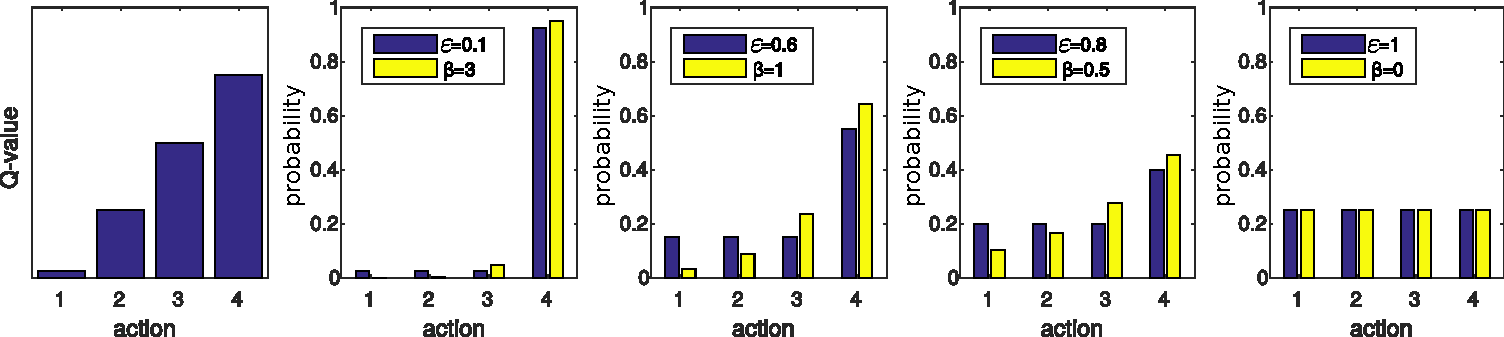
\includegraphics[width=\textwidth]{section4_fig23}

\paragraph{Optimistic initialization}
	\begin{itemize}
		\item initializing all Q-values with high 
			$Q_0 \geq \frac{r_\text{max}}{1-\gamma}$ directs exploration
		\vspace{1mm}
		\item unexplored actions are initially very attractive
		\vspace{1mm}
		\item Q-values are reduced until {\em exploitation} takes over
		\vspace{1mm}
		\item initially slower, but converges faster to the limit
		\vspace{1mm}
		\item can be applied 
			to SARSA($\lambda$) and Q-learning
	\end{itemize}
	
	\begin{minipage}{12cm}
		\begin{minipage}{4cm}
			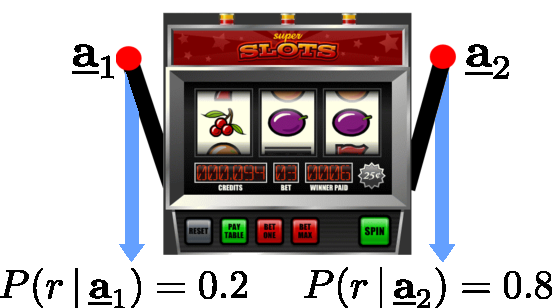
\includegraphics[width=\textwidth]{section4_fig24}
		\end{minipage}
		\begin{minipage}{8cm}
			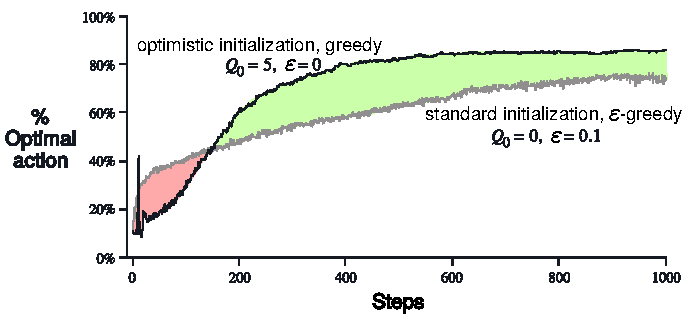
\includegraphics[width=\textwidth]{section4_fig25}
		\end{minipage}
	\end{minipage}
	
	{\hfill \footnotesize \citep[2-armed bandit task from][]{Sutton98}}

\paragraph{Model-based exploration: E$^3$ and R-MAX}
	\begin{enumerate}
		\vspace{-1mm}
		\item explore (e.g.~random-walk) until some states are visited often enough 
			\iitem{those states constitute the ``known set'' 
				$\bar{\Set S} \subset \Set X$}
		\vspace{1.5mm}
		\item estimate models of transitions and rewards in $\bar{\Set S}$
			\iitem{by counting observed transitions and rewards}
		\vspace{1.5mm}
		\item use these models to calculate 
			two Q-value functions in $\bar{\Set S}$:
			\begin{itemize}
				\item[``exploit'':] Q-value of {\em observed} rewards,
					transitions leaving $\bar{\Set S}$ yield no reward
				\vspace{0mm}
				\item[``explore'':] Q-value where {\em only}
					transitions leaving $\bar{\Set S}$ 
					yield a reward of $\frac{r_\text{max}}{1-\gamma}$
			\end{itemize}
		\vspace{1mm}
		\item in $\bar{\Set S}$, choose actions according 
			to the larger Q-value function
			\iitem{outside of $\bar{\Set S}$, continue random-walk
				and add explored states \\ to the known set $\bar{\Set S}$
				when visited sufficiently often}
	\end{enumerate}
	
	\vspace{2mm}
	\begin{minipage}{12.5cm}
		\hspace{4mm}
		\begin{minipage}{2.1cm}
			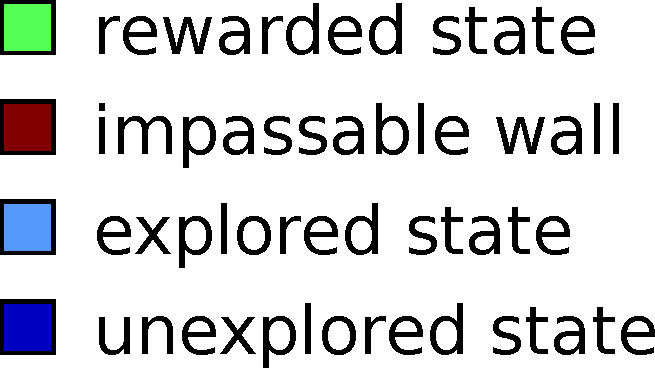
\includegraphics[width=\textwidth]{section4_fig26}
		\end{minipage}
		\hspace{2mm}
		\begin{minipage}{8.5cm}
			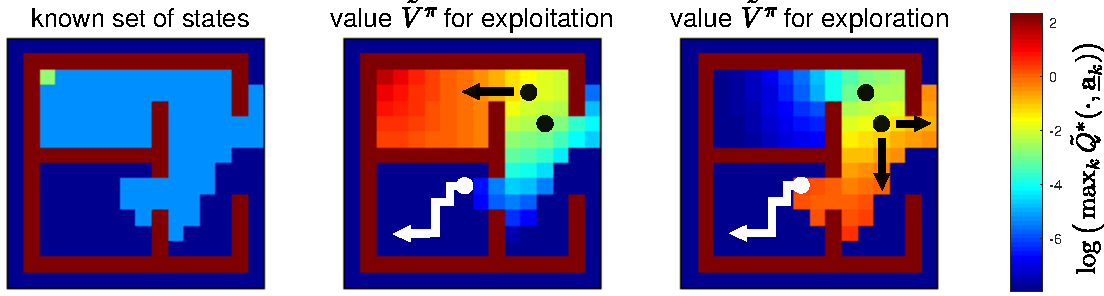
\includegraphics[width=\textwidth]{section4_fig27}
		\end{minipage}
	\end{minipage}
	
	%\vspace{8mm}
	{\footnotesize\citep[E$^3$,][]{Kearns02} 
		\hfill\citep[R-MAX,][]{Brafman02}}


% =============================================================================
\subsubsection{A Thorough Example: Mountain Car}
\paragraph{Mountain car}\mbox{}\\
	\begin{minipage}{12cm}
		\begin{minipage}{6.5cm}
			\begin{itemize}
				\item a car in a valley between mountains
					\iitem{$\Set X$: position and velocity}
				\vspace{2mm}
				\item agent drives the car
					\iitem{$\Set A$: forward, backward, nothing \\[-1.5mm]
						{\tiny (i.e., accelerate the car by $+a$, $-a$ and $0$)}}
				\vspace{2mm}
				\item dynamics are given by physics
					\iitem{deterministic {\color{trans}transition model $P$} 
					 \item gravitation but no friction}
				\vspace{2mm}
				\item{goal: reach right hilltop
					\iitem{{\color{reward}reward $r\kern-.5ex=\kern-.5ex0$}, 
							except {\color{reward}$r\kern-.5ex=\kern-.5ex1$} 
							at goal} }
			\end{itemize}
		\end{minipage}
		\hfill
		\begin{minipage}{5.5cm}
			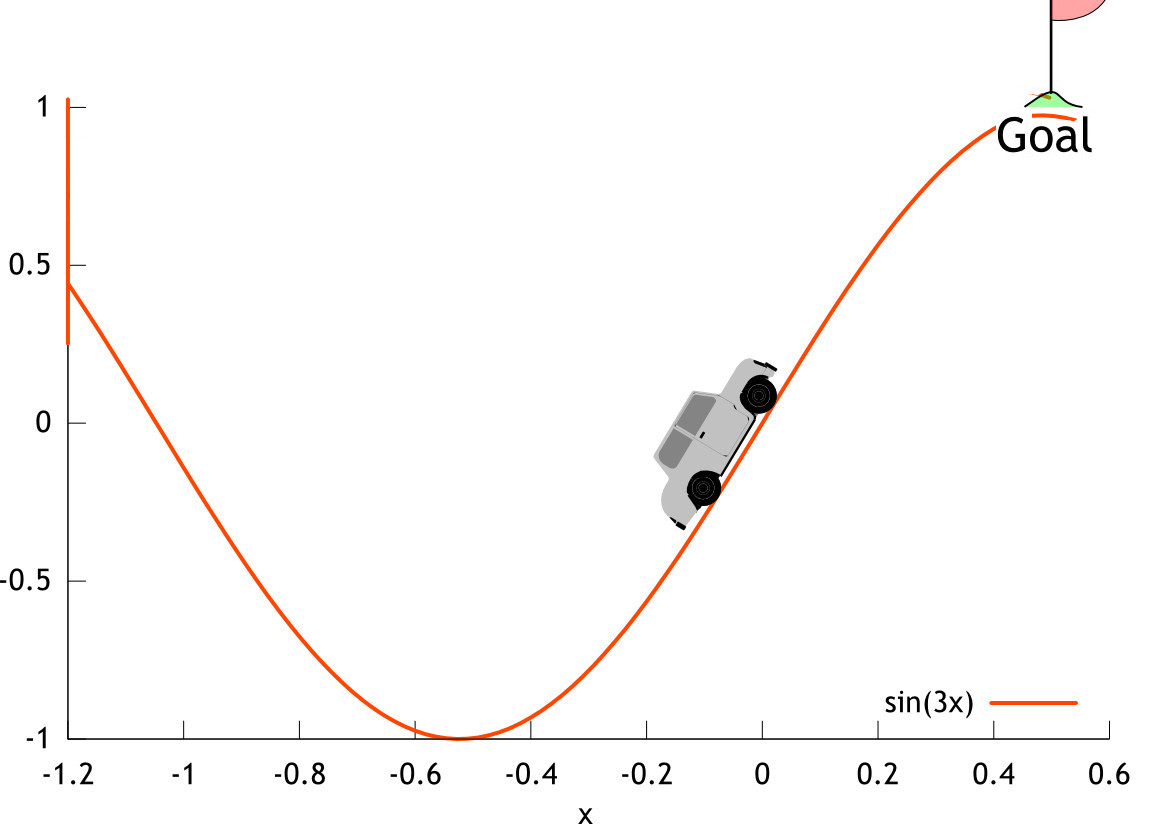
\includegraphics[width=\textwidth]{mountaincar2.jpg}
		\end{minipage}
	\end{minipage}
	
	\vspace{2mm}
	\iitem{exploration/exploitation is performed in {\bf episodes}
		\iitem{start motionless at the bottom
		 \item end after 1000 steps or when the goal is reached
		 \item very few episodes with random control reach the goal}}

\paragraph{Q-learning: Development of the value function}
	\iitem{Q-learning with optimistic initialization 
		and $\epsilon$-greedy sampling policy
		\iitem{$\epsilon=0, Q_0=10, \lr=0.5, \gamma=0.9$, 
			discretization in $50 \times 50$ states}}
	\vspace{20cm}
	

		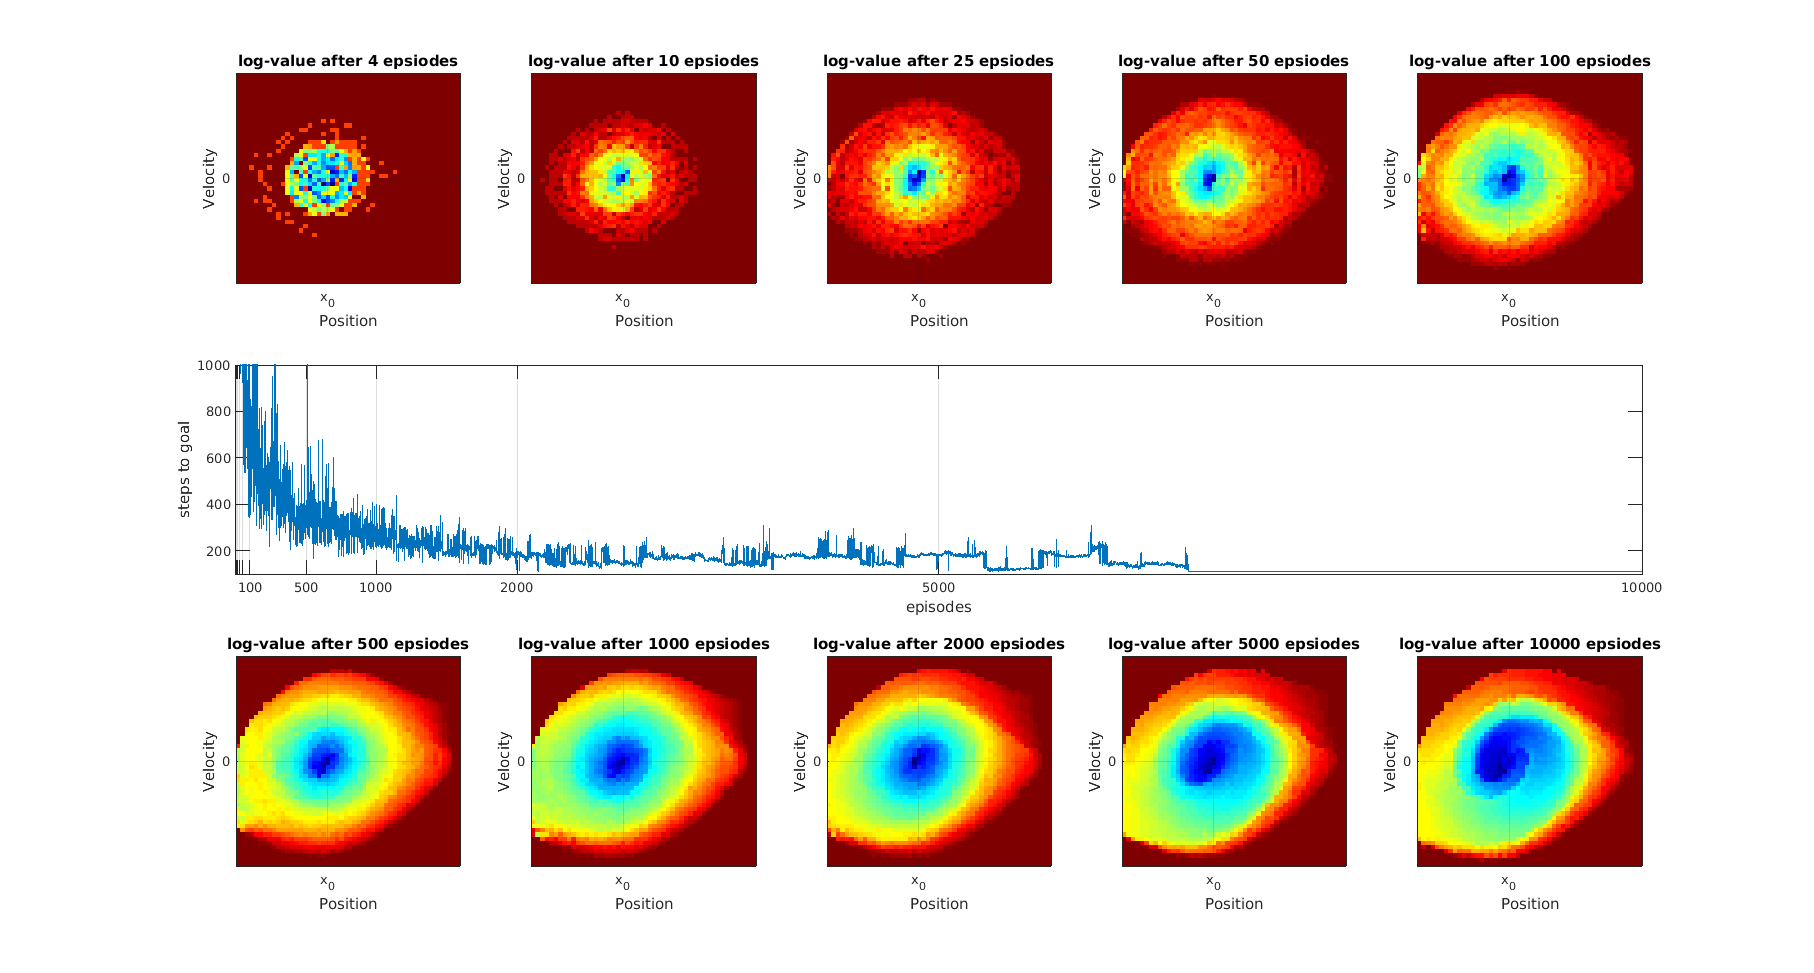
\includegraphics[width=12.5cm]{mountaincar_qlearning_overtime.png}


\paragraph{Parcellation of state space}
	%\iitem{task is continuous, state can be discretized freely}
	\iitem{finer grids lead to better policies, 
			but learning requires more episodes}
	\iitem{coarse discretizations 
			may fail to learn a good policy}

	\vspace{2mm}
	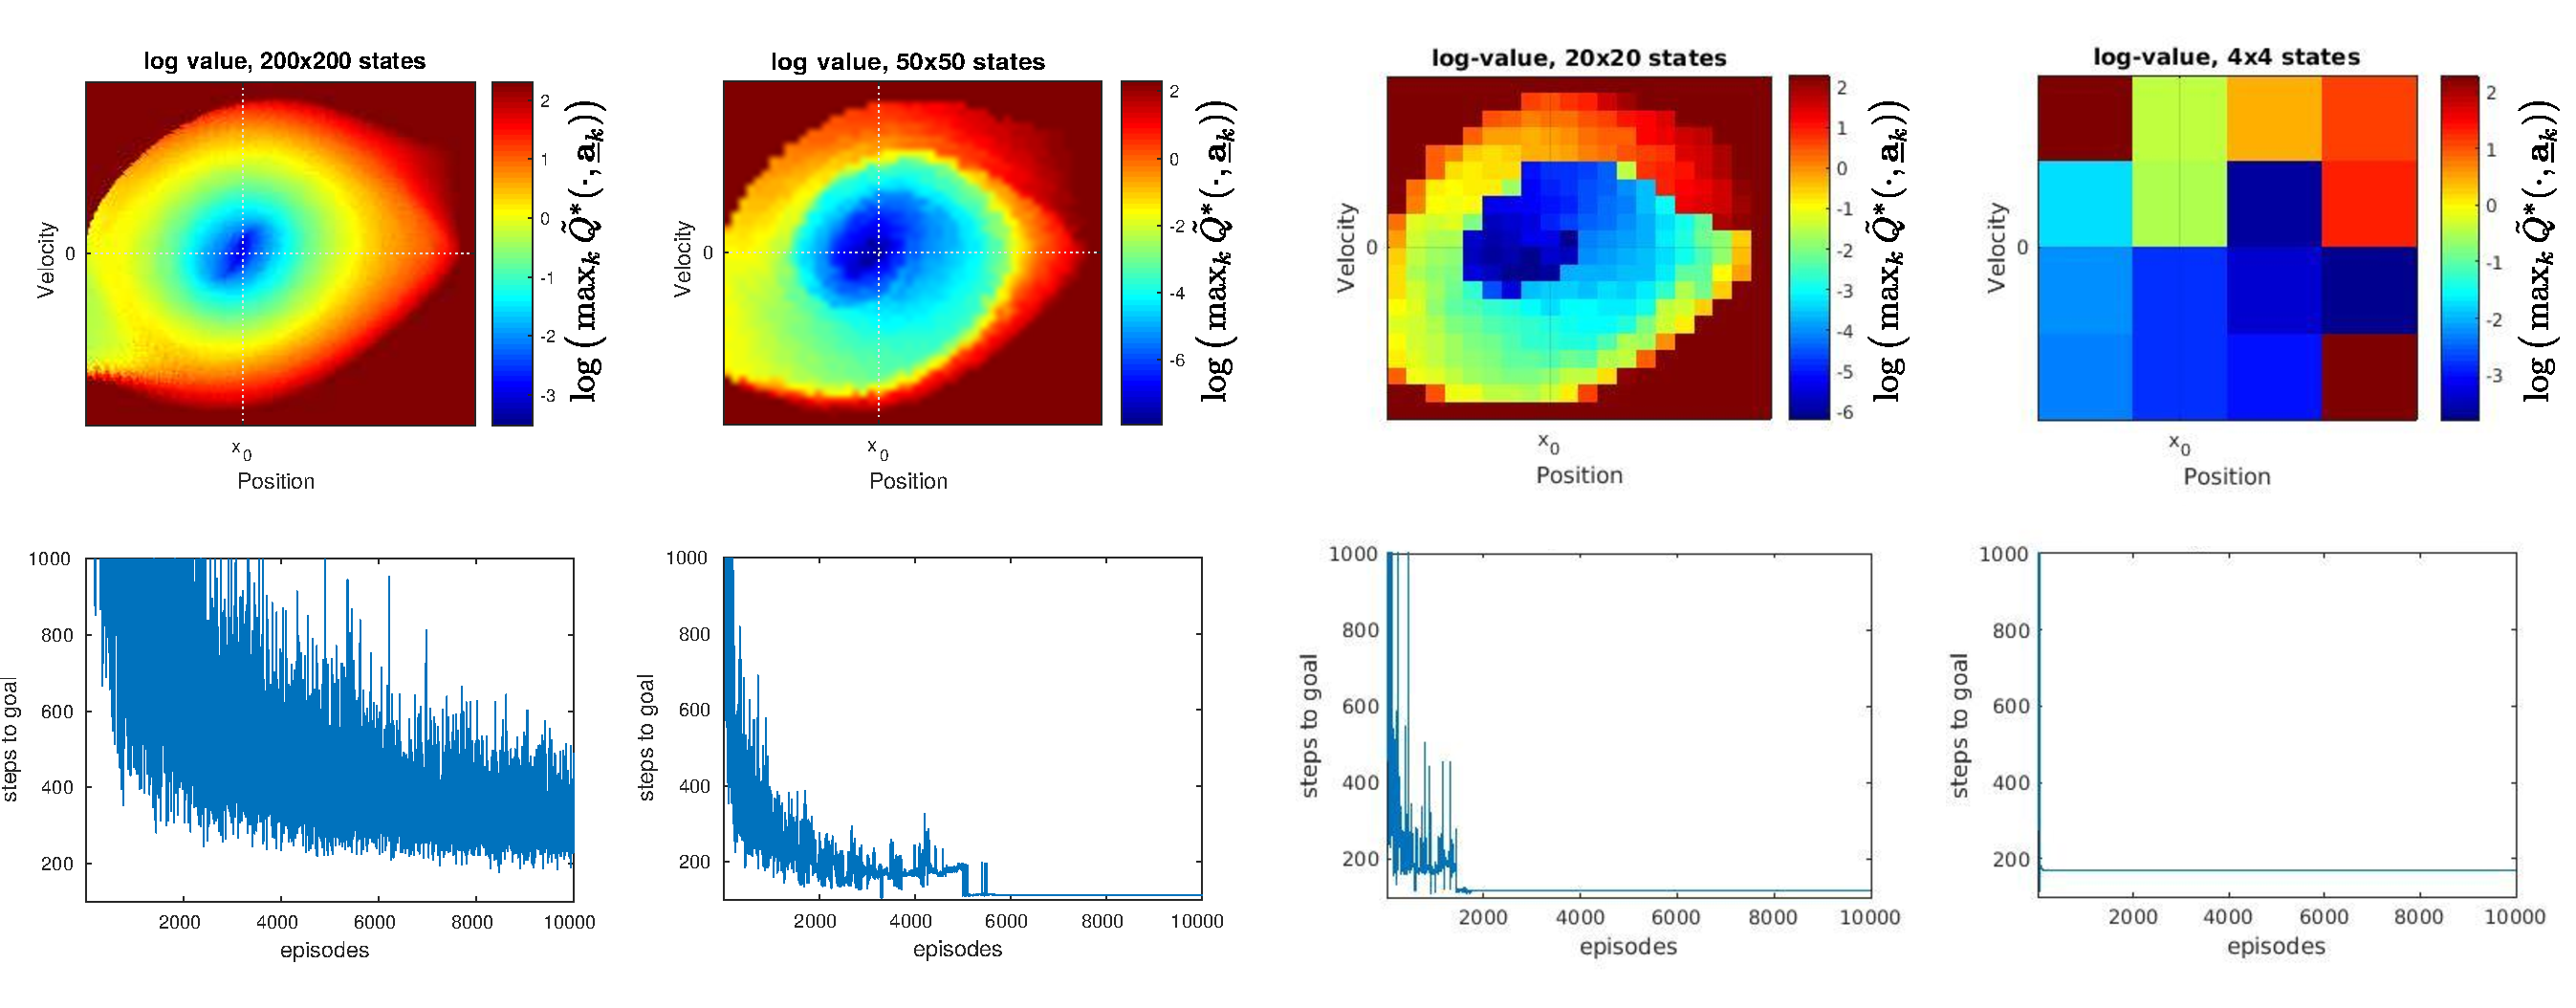
\includegraphics[width=\textwidth]{section4_fig28.pdf}

\paragraph{Optimistic initialization}
	\iitem{without optimistic initialization, 
			$\varepsilon$-greedy Q-learning fails
		\iitem{observed reward must be propagated over 100+ time steps
		 \item $\varepsilon$-greedy does not reach the goal 
		 	often enough (for any $\varepsilon$)}}
	\iitem{small initial $Q_0 = \frac{r_\text{max}}{1-\gamma}$ converges faster, 
		but yields suboptimal policies}
	
	\vspace{-1mm}
	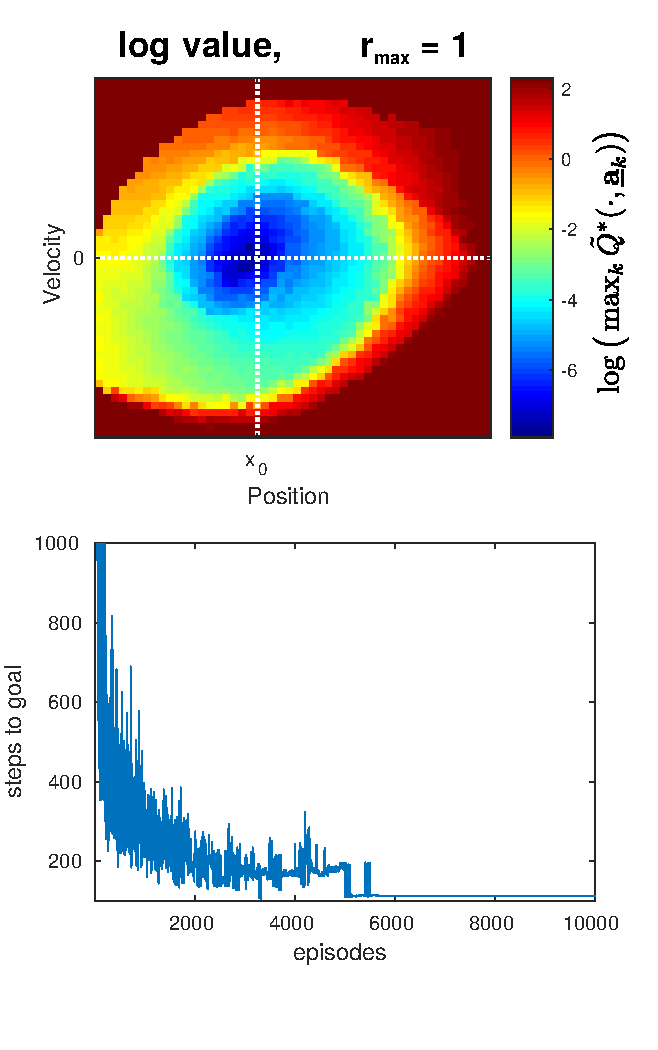
\includegraphics[width=3.8cm]{section4_fig29}
	\hfill
	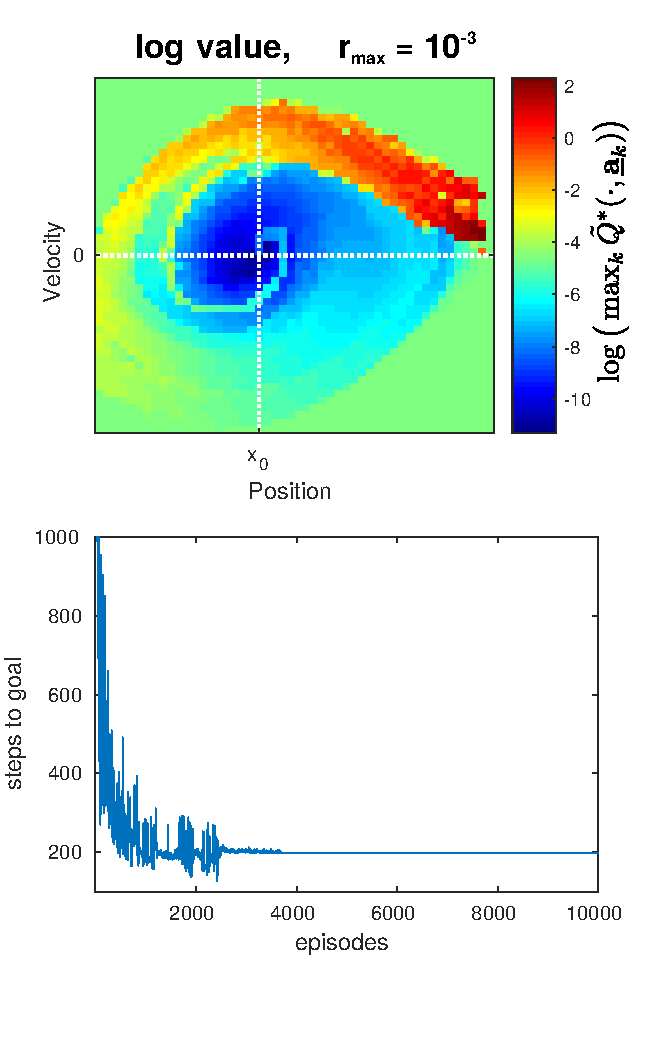
\includegraphics[width=3.8cm]{section4_fig30}
	\hfill
	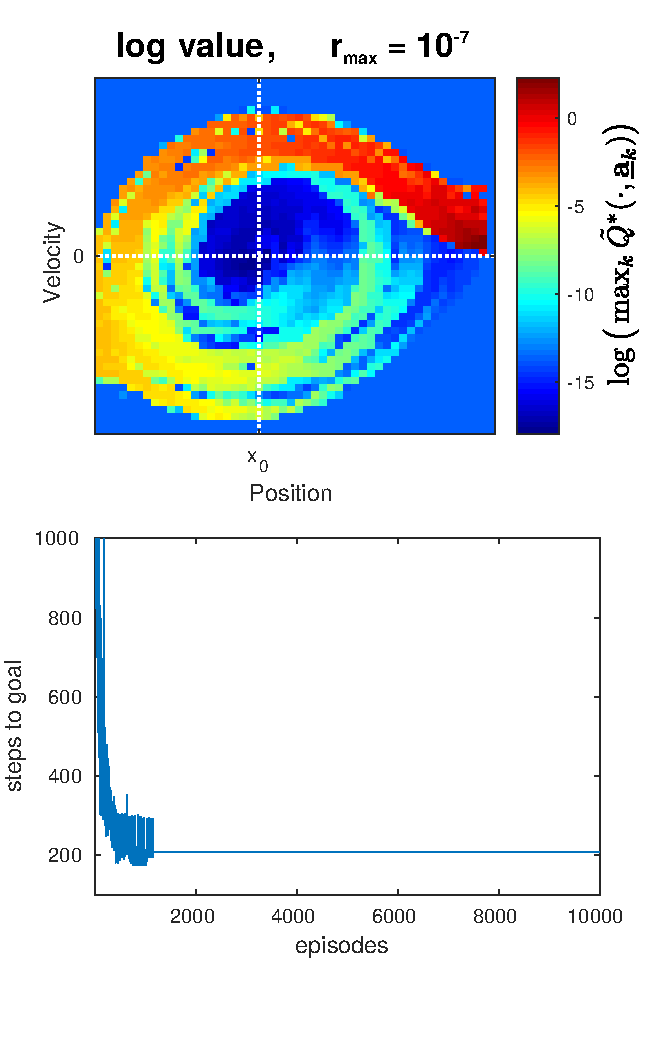
\includegraphics[width=3.8cm]{section4_fig31}
	
\paragraph{Non-deterministic transitions}
	\iitem{i.i.d.~wind $\vec a \pm|\omega_t|$\, \quad with 
	  $\omega_t \sim \Set N(0, \sigma^2)$, $\sigma = \frac{2}{3}$
	}

	\vspace{2mm}
	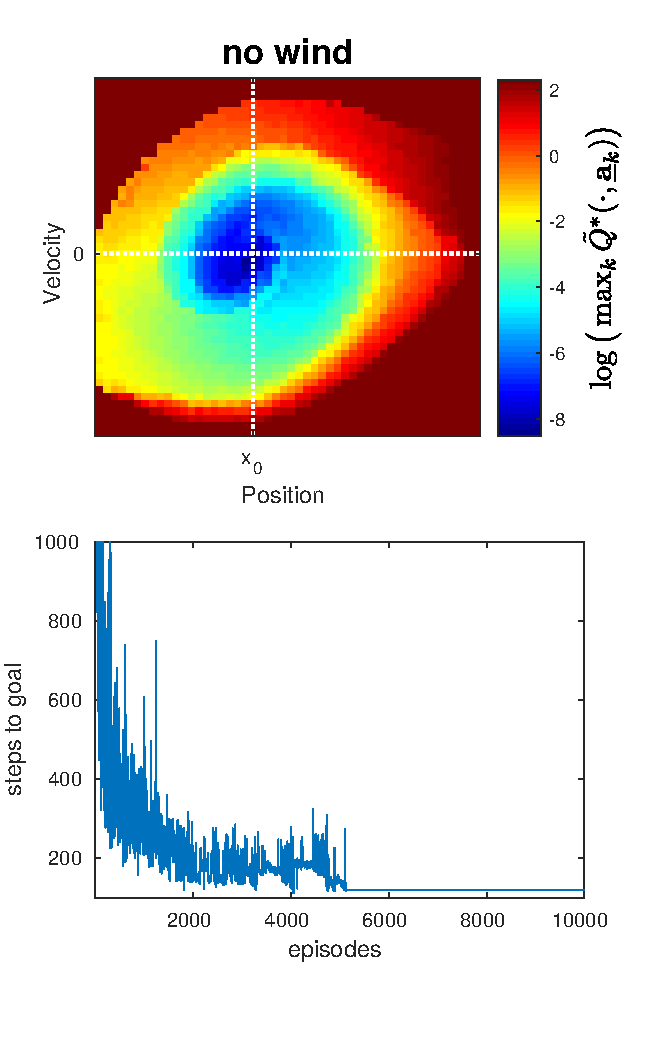
\includegraphics[width=4cm]{section4_fig32}
	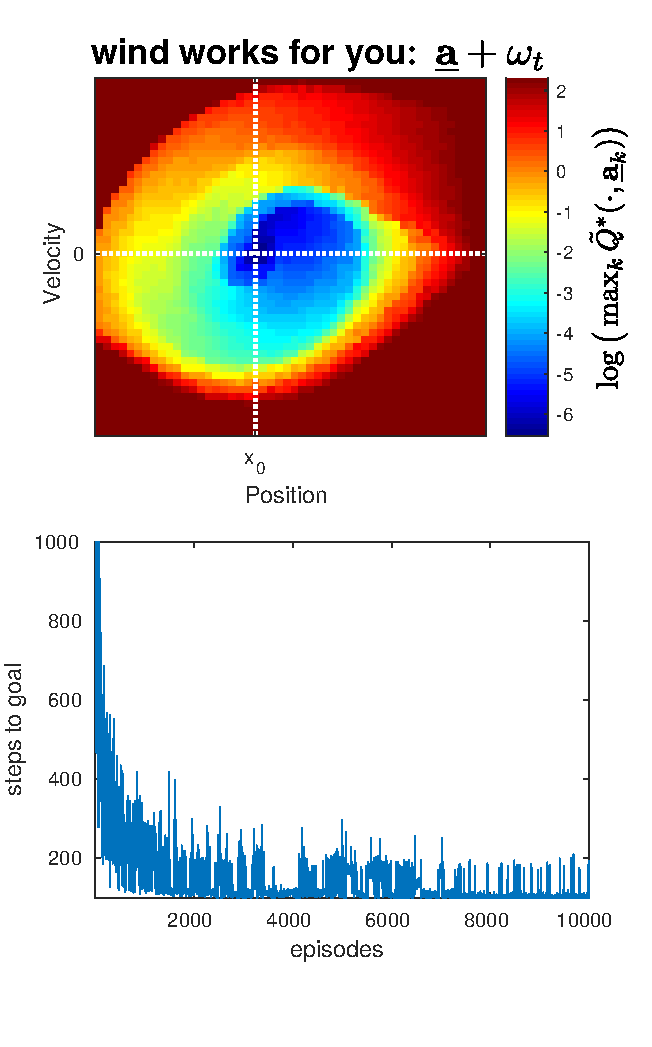
\includegraphics[width=4cm]{section4_fig33}
	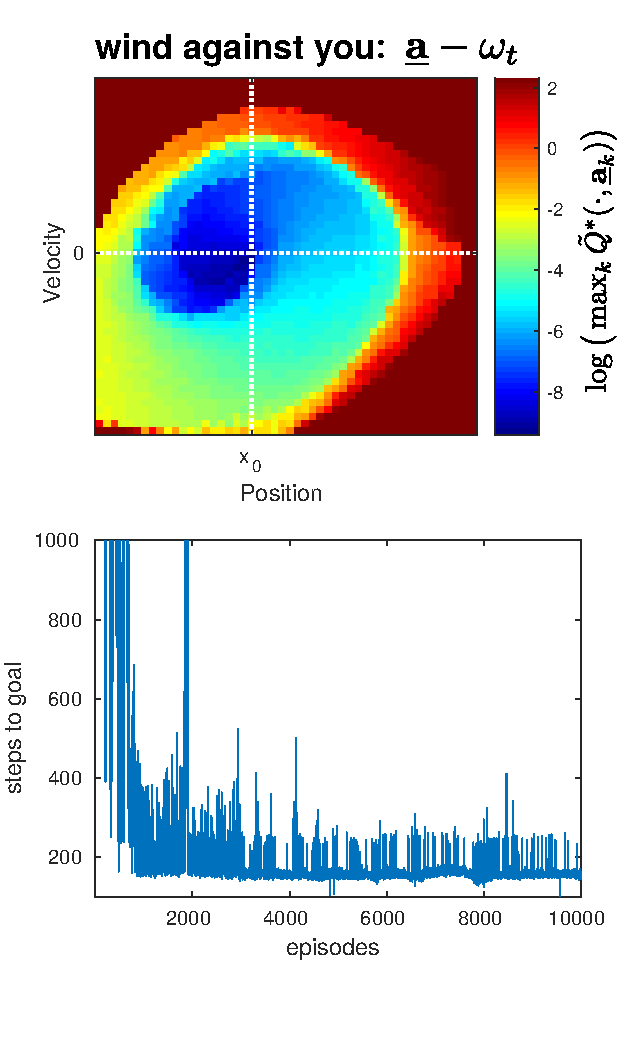
\includegraphics[width=4cm]{section4_fig34}

% =============================================================================
\subsubsection{Approximate RL}
\paragraph{Real-world application of RL}\mbox{}\\
	\begin{minipage}{\textwidth}
		\begin{minipage}{0.8\textwidth}
			\begin{itemize}
				\item  realistic state spaces can be huge 
					\iitem{\footnotesize e.g.~game of GO has $3^{19 \times 19} 
						\approx 10^{172}$ states \\ \citep{Silver16}}
				\vspace{4mm}
				\item real world states/actions are often continuous
					\iitem{\footnotesize e.g.~autonomous helicopter control 
						\citep{Abbeel07}}
			\end{itemize}
	
			\vspace{0mm}
			\begin{center}
				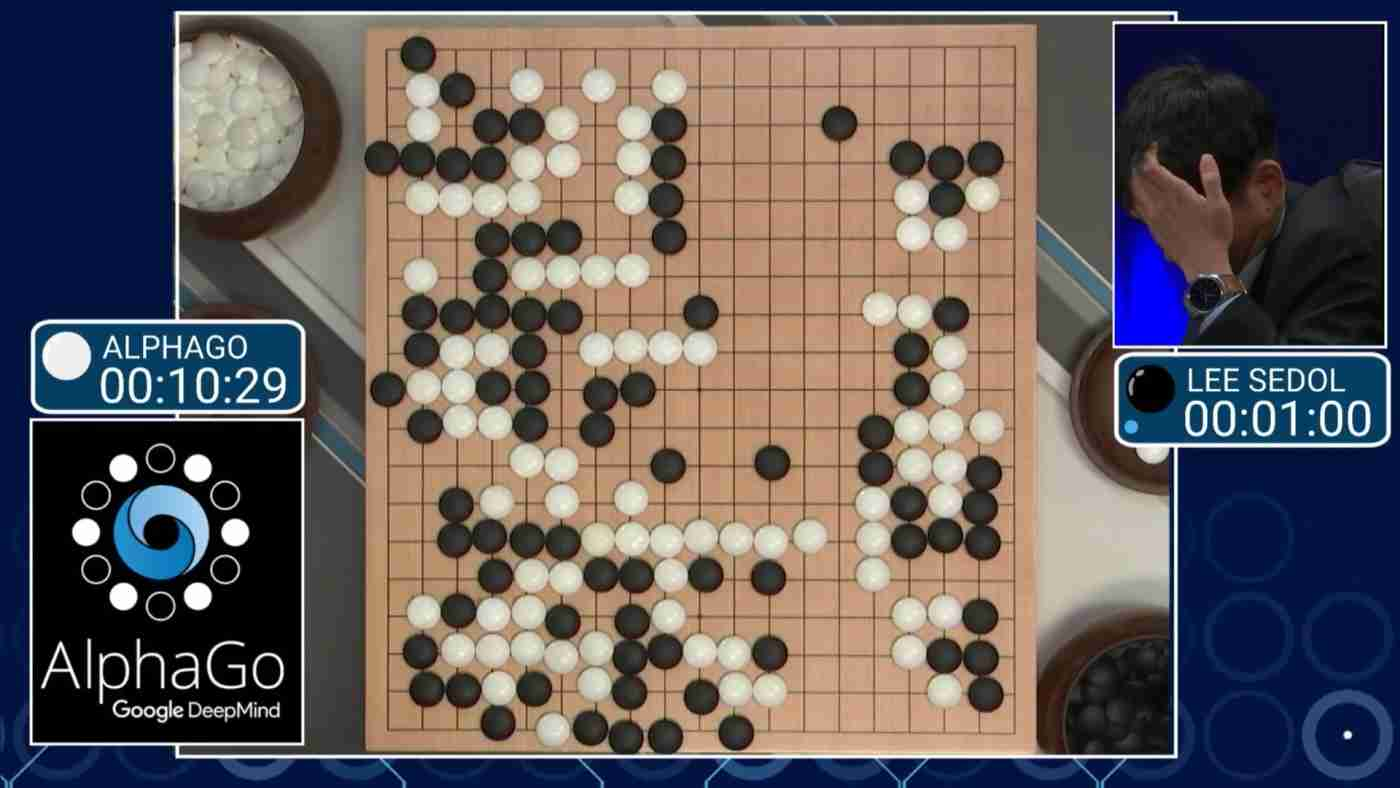
\includegraphics[height=2.8cm]{alphaGO.jpg}
			\end{center}
		\end{minipage}
		\begin{minipage}{.19\textwidth}
			
				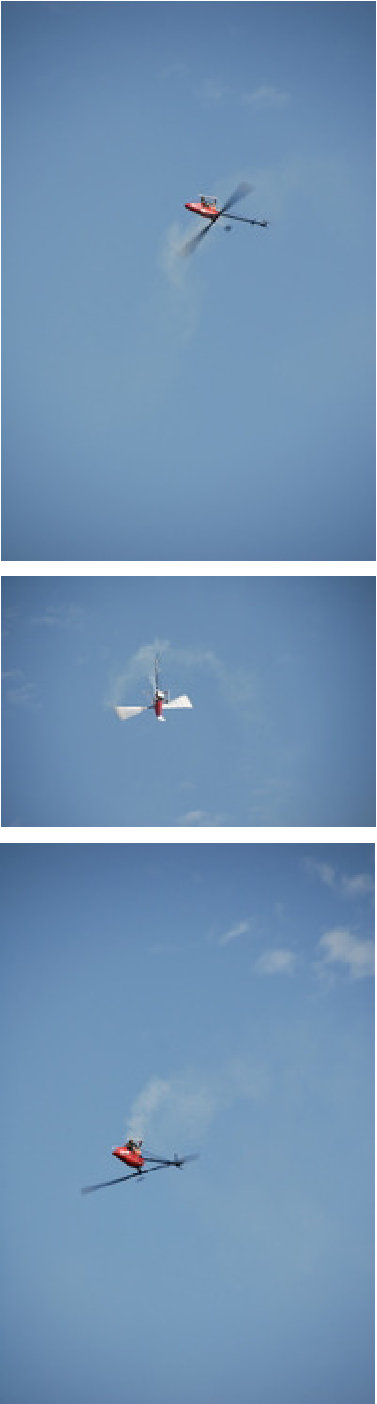
\includegraphics[height=7.6cm]{helicopter.pdf}
			
		\end{minipage}
	\end{minipage}

\paragraph{Value function approximation}
	\begin{itemize}
		\item previous methods require values for all states
			\iitem{continuous state spaces must be discretized}
		\vspace{4mm}
		\item often impossible to visit every state-action pair
		\vspace{4mm}
		\item use function approximation to generalize Q-values
			 \vspace{.5mm}
			 \iitem{training set $\{\vec x^{(t)}, \vec a^{(t)}, r_t \}_{t=0}^p$ 
					drawn by an ergodic Markov chain 
			 \vspace{.5mm}
			 \item model classes: {\em linear functions},
			 		{\em multi-layer perceptrons}, \ldots}
		\begin{center}
			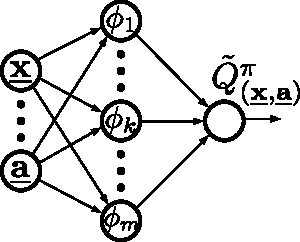
\includegraphics[height=3cm]{section4_fig35}
			 \hspace{2cm}
			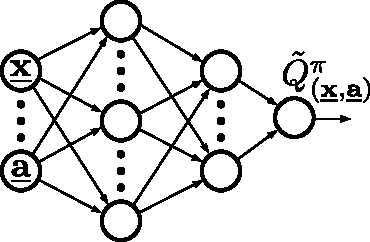
\includegraphics[height=3cm]{section4_fig36} \\
			basis-function approach 
			\hspace{20mm}
			deep neural network
			\hspace{14mm}$ $
		\end{center}
	\end{itemize}
\paragraph{Minimization of Bellman residuals}
	\begin{itemize}
		\item quadratic error with parameterized \\function 
				$\tilde Q^\pi(\vec x, \vec a; \vec w)$
			\vspace{1mm}
			 $$ \hspace{-1.5cm}
			 	E^T_\text{\tiny BRM} \quad=\quad \smallfrac{1}{2p}
			 	\sum_{t=0}^{p-1} \Big( \underbrace{ 
			 		\overbrace{
			 		{\color{reward}r_t} 
			 			+ \gamma \tilde Q^\pi 
			 				({\color{trans}\vec x^{(t+1)}, 
			 					\vec a^{(t+1)}}; \vec w)
			 		}^{\text{target value for }\tilde Q^\pi 
			 				(\vec x^{(t)}, \vec a^{(t)}; \vec w)}	
		 			- \; \tilde Q^\pi(\vec x^{(t)}, \vec a^{(t)}; \vec w)
			 	}_{\text{TD-error}\;\Delta Q_t}\Big)^2
			 $$
		\vspace{4mm}
		\item minimize $E^T_{\text{BRM}}$ e.g.~with gradient descend
	\end{itemize}
	\begin{center}
		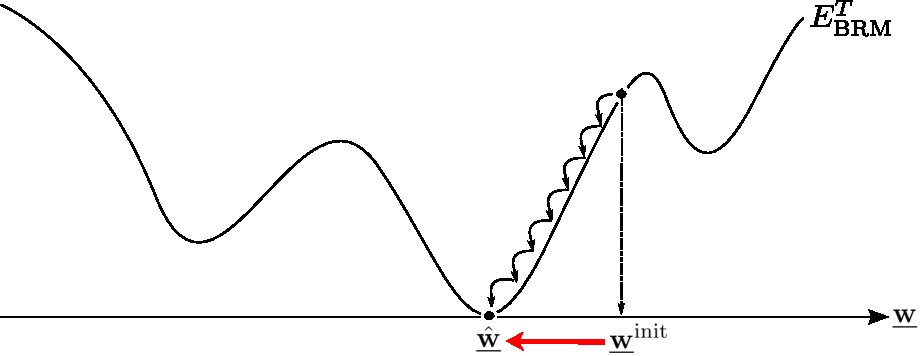
\includegraphics[height=3cm]{section4_fig38}
	\end{center}	
\begin{itemize}
		%\item two possible gradients for {\em online learning} 
		\vspace{2mm}
		\item {\bf residual gradient} for gradient descend \\[1mm]
			$\frac{\partial(\Delta Q_t)^2}{\partial \vec w}
			\quad=\quad -2 \Delta Q_t \,\Big(
				\frac{\partial \tilde Q^\pi
					(\vec x^{(t)}, \vec a^{(t)};\vec w)}{\partial \vec w}
				- \gamma \frac{\partial \tilde Q^\pi 
					(\vec x^{(t+1)}, \vec a^{(t+1)}; \vec w)}{\partial \vec w}
			\Big)$ 
			
			\iitem{moves $\tilde Q^\pi(\vec x^{(t)}, \vec a^{(t)}; \vec w)$ towards 
				${\color{reward}r_t} + \gamma 
				\tilde Q^\pi ({\color{trans}\vec x^{(t+1)}, \vec a^{(t+1)}}; \vec w)$
			 \vspace{1mm}
			 \item but also 
				$\tilde Q^\pi ({\color{trans}\vec x^{(t+1)},\vec a^{(t+1}}; 
				\vec w)$ towards 
				$\frac{1}{\gamma}\big(\tilde Q^\pi(\vec x^{(t)}, \vec a^{(t)}; \vec w) 
				- {\color{reward}r_t}\big)$
			 \vspace{1mm}
			 \item converges very slowly \citep{Baird95}}
			 
		\vspace{2mm}
		\item  {\bf semi-gradient} approximates gradient descend \\[1mm]
				$	\frac{\partial (\Delta Q_t)^2}{\partial\vec w} 
				 	\quad\approx\quad -2 \Delta Q_t \, 
					\smallfrac{\partial 
						\tilde Q^\pi(\vec x^{(t)}, \vec a^{(t)}; \vec w)}
						{\partial \vec w}$
			
				\begin{itemize}
					\item assume target ${\color{reward}r_t} 
						+ \gamma \,
						\tilde Q^\pi({\color{trans}\vec x^{(t+1)},
							\vec a^{(t+1})}; \vec w)$ 
						is independent of $\vec w$ 
					\vspace{1mm}
					\item converges faster than residual gradients \citep{Gordon95}
				\end{itemize}
				\vspace{5mm}
			
	\end{itemize}
	
	\vspace{-4mm}
	{\footnotesize\hfill\citep[see][]{Sutton98}}

\paragraph{Online semi-gradient descent (on-policy)}	
	\begin{eqnarray*}
		\vec w^{(i+1)} &=&
			\vec w^{(i)} \;-\; \lr \,
			\smallfrac{\partial 
				e^{(t)}_\text{BRM}}
				{\partial \vec w} \\[4mm]
	 	e^{(t)}_\text{\tiny BRM} &=& 
	 		\smallfrac{1}{2}
			 	\Big( \underbrace{ 
			 		{\color{reward}r_t} 
			 			+ \gamma \tilde Q^\pi 
			 				({\color{trans}\vec x^{(t+1)}, \vec a^{(t+1)}}; \vec w)	
		 			- \; \tilde Q^\pi(\vec x^{(t)}, \vec a^{(t)}; \vec w)
			 	}_{\text{TD-error}\;\Delta Q_t}\Big)^2
	\end{eqnarray*}
	
	\vspace{2mm}
	\begin{itemize}
		\item semi-gradient \quad
				$	\frac{\partial e^{(t)}_\text{BRM}}{\partial\vec w} 
				 	\quad\approx\quad -\Delta Q_t \, 
				 	\underbrace{\smallfrac{\partial 
						\tilde Q^\pi(\vec x^{(t)}, \vec a^{(t)}; \vec w)}
						{\partial \vec w}
					}_{\kern-10ex\text{backpropagation}\kern-10ex}$
		\vspace{4mm}
		\item {\em on-policy} value estimation 
			\iitem{converges for basis function networks \citep{Sutton98}
			 \item may not converge for non-linear functions (like MLP)}
	\end{itemize}

\paragraph{Online semi-gradient descent (off-policy)}
	\begin{eqnarray*}
		\vec w^{(i+1)} &=&
			\vec w^{(i)} \;-\; \lr \,
			\smallfrac{\partial 
				e^{(t)}_\text{BRM}}
				{\partial \vec w} \\[4mm]
	 	e^{(t)}_\text{\tiny BRM} &=& 
	 		\smallfrac{1}{2}
			 	\Big( \underbrace{ \scriptstyle
			 		{\color{reward}r_t} 
			 			\;+\; \gamma {\color{policy}\sum\limits_{k=1}^{A} 
			 				\kern-.5ex\pi(\vec a_k|{\color{trans}\vec x^{(t+1)}})} \,
			 			\tilde Q^\pi({\color{trans}\vec x^{(t+1)}},\,
			 				{\color{policy}\vec a_k}; \vec w)	
		 			\;-\; \; \tilde Q^\pi(\vec x^{(t)},\, \vec a^{(t)}; \vec w)
			 	}_{\text{TD-error}\;\Delta Q'_t}\Big)^2
	\end{eqnarray*}
	
	\vspace{2mm}
	\begin{itemize}
		\item semi-gradient \quad
				$	\frac{\partial e^{(t)}_\text{BRM}}{\partial\vec w} 
				 	\quad\approx\quad -\Delta Q'_t \, 
					\underbrace{\smallfrac{\partial 
						\tilde Q^\pi(\vec x^{(t)}, \vec a^{(t)}; \vec w)}
						{\partial \vec w}
					}_{\kern-10ex\text{backpropagation}\kern-10ex}$
		\vspace{4mm}
		\item online {\em off-policy} value estimation 
			using semi-gradients may not
			\iitem{for all known model classes \citep{Baird95,Tsitsiklis97}}
	\end{itemize}

\paragraph{Gradient descend on Markov chains}
	\vspace{6mm}	
	\begin{itemize}
		\item online gradient descend on Markov chains often fails:
			\begin{itemize}
				\item gradient updates can influence value 
					predictions for all states
				\vspace{1mm}
				\item the data is not drawn i.i.d.~from 
					a stationary distribution %(Section 1.4, p.~4)
			\end{itemize}
		\vspace{6mm}
		\item solution: {\bf experience replay}:
			\iitem{sampling state-action pairs from 
				long ergodic Markov chains is equivalent 
				to sampling state-action pairs 
				from the underlying \\ stationary distribution
					{\footnotesize (Section 4.1, p.~26)}
		}
	\end{itemize}
	
\paragraph{Semi-gradient Q-learning}

	\iitem{model class: multi-layer perceptrons
			$\tilde Q^{*}(\vec x, \vec a; \vec w)$} 
	$$
		e^{(t)}_\text{\tiny BRM} \quad = \quad 
		\smallfrac{1}{2} 
		\Big( \underbrace{ \overbrace{ {\color{reward}r_t} 
			+ \gamma {\color{policy}\max_{\vec a' \in \Set A}}\,
				\tilde Q^*({\color{trans}\vec x^{(t+1)}}, 
					{\color{policy}\vec a'}; \vec w)
				}^{\text{target of }\tilde Q^*
					(\vec x^{(t)}, \, \vec a^{(t)}; \vec w)}
			\;-\; \tilde Q^*(\vec x^{(t)}, \vec a^{(t)}; \vec w)
		}_{\text{TD-error }\Delta Q^*_t} \Big)^2
	$$
	\vspace{2mm}
	\begin{itemize}
		\item semi-gradient \quad 
				$	\frac{\partial e^{(t)}_\text{BRM}}{\partial\vec w} 
				 	\quad=\quad -\Delta Q^*_t \;
					\underbrace{\smallfrac{\partial 
						\tilde Q^*(\vec x^{(t)}, \vec a^{(t)}; \vec w)}
						{\partial \vec w} }_{\text{backpropagation}} $
		\vspace{2mm}
		\item gradient descend with i.i.d.~samples 
			from {\em experience replay} buffer
			\iitem{reuses all (or the last $p$) observed samples}
		\vspace{4mm}
		\item semi-gradient Q-learning is {\em off-policy} 
			and may not converge
%		\vspace{4mm}
%		\item it is in praxis more stable to approximate 
%			the Bellman operator $\hat B^*$ 
	\end{itemize}


% -----------------------------------------------------------------------------
\paragraph{Neural fitted Q-learning (NFQ)} \label{NFQ}
	\begin{itemize}
		\item approximate Q-learning operator $\hat B^*$ with MLP
			\vspace{1mm}
			\begin{itemize}
				\item off-policy {\em batch learning} 
					using {\em experience replay}
				\vspace{1mm}
				\item determine $\vec w^{(i+1)}$ by regression 
					of targets $y_T^{(t)}$
			\end{itemize}
			\vspace{2mm}
			$$ \hspace{-6mm}
				y_T^{(t)} \quad:=\quad 
				\hat B^*[\tilde Q^*(\vec x^{(t)}, \vec a^{(t)}; \vec w^{(i)})]
				\quad=\quad {\color{reward}r_t}
				\;+\; \gamma \, {\color{policy}\max_{\vec a' \in \Set A}}\,
				\tilde Q^*{({\color{trans}\vec x^{(t+1)}}, 
					{\color{policy}\vec a'}; \vec w^{(i)})} 
			$$
			%\vspace{2mm}			
		\item any MLP regression algorithm can be used
	\end{itemize}
	
	NFQ algorithm: \citep{Riedmiller05} \\
		initialize $\vec w^{(0)}$ randomly \\
		\While{$\vec w^{(i)}$ not converged}{
			\For{$t \in \{1,\ldots,p-1\}$}{
				$y_T^{(t)} \leftarrow {\color{reward}r_t} + \gamma \, 
				{\color{policy}\max\limits_{\vec a' \in \Set A}}
				\tilde Q^*({\color{trans}\vec x^{(t+1)}}, 
				{\color{policy}\vec a'}; \vec w^{(i)})$ \\[-5mm]
			}
			\vspace{-1mm}
			$\vec w^{(i+1)} \leftarrow \text{\texttt{regression}}
				\Big(\Big\{\Big[\kern-.75ex\begin{array}{c}
					\vec x^{(t)} \\[-1mm] \vec a^{(t)}
				\end{array}\kern-1.25ex\Big], y_T^{(t)} 
				\Big\}_{\kern-.5ext=0}^{\kern-.5exp-1} \Big)$
			\vspace{-1mm}
		}

% =============================================================================
\subsubsection{Least-Squares RL}
\paragraph{Projected Bellman operator}\citep[see][]{Bertsekas07}
	\begin{itemize}
		\item \small linear model $\tilde Q^\pi(\vec x,\vec a; \vec w) 
				= \vec w^\top \vec \phi(\vec x,\vec a)$ 
			with $\phi_i: \Set X\kern-.5ex\times\kern-.5ex \Set A \to \R$
		\vspace{1mm}
		\item approximate Bellman operator 
			$B^\pi[\tilde Q^\pi(\vec x^{(t)}, \vec a^{(t)}; \vec w^{(i)})]$
	\end{itemize}
\begin{eqnarray*} \hspace{-1mm}
		\min_{\vec w^{(i+1)}} \kern-1exE^T_\text{BRM}  
		\kern-1ex&=&\kern-1ex
		\min_{\vec w^{(i+1)}} \smallfrac{1}{2p} \sum_{t=0}^{p-1} 
			\Big( \overbrace{\underbrace{{\color{reward}r_t} 
				+ \gamma \tilde Q^\pi({\color{trans}\vec x^{(t+1)}}\kern-1ex,
					{\color{policy}\vec a^{(t+1)}}; \vec w^{(i)})
				}_{\text{independent of }\vec w^{(i+1)}}
				}^{\text{target }B^\pi[\tilde Q^\pi(\vec x^{(t)}, \vec a^{(t)}; 
					\vec w^{(i)})]}
			- \tilde Q^\pi(\vec x^{(t)}\kern-1ex, \vec a^{(t)}; \vec w^{(i+1)})
			\Big)^2 \\[-2mm] 
		\frac{\partial E^T_\text{BRM}}{\partial \vec w^{(i+1)}} 
		\kern-1ex&=&\kern-1ex
			\overbrace{\smallsum{t=1}{p-1} 
				\vec\phi_{(\vec x^{(t)}\kern-.2ex, \vec a^{(t)})}
				\vec\phi_{(\vec x^{(t)}\kern-.2ex, \vec a^{(t)})}^\top
			}^{\vec C} \vec w^{(i+1)}
			- \; \overbrace{\smallsum{t=1}{p-1}
				\vec\phi_{(\vec x^{(t)}\kern-.2ex, \vec a^{(t)})} \, 
					{\color{reward}r_t}
				}^{{\color{reward}\vec b}} \\[-1mm]
			&& - \; \gamma \underbrace{\smallsum{t=1}{p-1} 
				\vec\phi_{(\vec x^{(t)}\kern-.2ex, \vec a^{(t)})}
				\vec\phi_{({\color{trans}\vec x^{(t+1)}}\kern-.2ex,
					{\color{policy}\vec a^{(t+1)}})}^\top
					}_{{\color{trans}\vec D^\pi}} \vec w^{(i)} 
			\quad \stackrel{!}{=} \quad 0 \\[0mm] 
		\vec w^{(i+1)} &=&  
			\vec C^{-1} \big( {\color{reward}\vec b}
			+ \gamma {\color{trans}\vec D^\pi} \vec w^{(i)} \big)
		\quad=:\quad
			\tilde B^\pi\big[\vec w^{(i)}\big]
	\end{eqnarray*}
\begin{itemize}
		\item<3> {\bf projected Bellman operator} $\tilde B^\pi$
				is affine transformation of $\vec w^{(i)}$
	\end{itemize}	

\paragraph{Least-squares temporal difference learning (LSTD)}
	\vspace{-2mm}
	\begin{itemize}
		\item fixed point $V(\vec x; \vec w^*) 
			= \tilde B^\pi[V(\vec x; \vec w^*)]$ 
			is the LSTD solution \citep[defined by][]{Bradtke96}
	\end{itemize}
	$$
		\vec w^* \quad=\quad \big( \vec C 
			- \gamma {\color{trans}\vec D^\pi} \big)^{-1} 
			{\color{reward}\vec b}
			\quad=\quad  \big( \vec I - 
			\gamma \, { \color{blue} \underbrace{\vec C^{-1} 
				\vec D^\pi}_{\tilde{\vec P}^\pi}}
			\big)^{-1} {\color{reward} \underbrace{\vec C^{-1} \vec b
				}_{\tilde{\vec r}}
		}
	$$
\begin{itemize}
		\item  LSTD solution is fixed point of least-squares 
			models $\color{blue}\tilde{\vec P}^\pi$ 
			and $\color{reward}\tilde{\vec r}$ \citep[see][]{Parr08}
			\vspace{.5mm}
			\iitem{discrete batch value estimation is special case of LSTD}
		\vspace{4mm}
		\item on-policy LSTD finds a fixed point close to $V^\pi$
			\vspace{.5mm}
			\begin{itemize}
				\item $\tilde B^\pi$ is a contraction mapping
					and the approximation error is bounded\footnote{
						in a $L_2$ norm weighted with the 
						{\em steady state distribution} $P_\text{ssd}$
						%$\|\vec v\|_{P_\text{ssd}} 
						%= \sum_i P_\text{ssd}(\vec x_i) \, v_i^2$
					}
			\end{itemize}
			\vspace{2mm}
			$$ \hspace{-1cm}
				\Big\|V^\pi - \vec\phi^\top \vec w^* \Big\|_{P_\text{ssd}}
				\quad\leq \quad 
				\smallfrac{1}{\sqrt{1-\gamma^2}}
				\Big\| V^\pi - \underbrace{\vec\phi^\top 
				\E\big[\vec \phi \,\vec \phi^\top\big] \,
				\E\big[\vec \phi V^\pi\big]
				}_{\text{value projected on $\vec\phi$}}\Big\|_{P_\text{ssd}}
			$$ \citep[proven by][]{Tsitsiklis97}
	\end{itemize}

\paragraph{Least-squares policy iteration (LSPI)}

	\begin{itemize}
		\item policy iteration with LSTD as {\em off-policy} Q-value estimator
			\vspace{1mm}
			\iitem{given training set 
				$\{\vec x^{(t)}, \vec a^{(t)}, r_t\}_{t=0}^p$
				and bases $\phi_i: \Set X \times \Set A \to \R$
			 \vspace{1mm}
			 \item greedy policy chooses action $\vec a'^{(t+1)}$ 
			 	for each sample $\vec x^{(t+1)}$}
	\end{itemize}
	\vspace{-1mm}
LSPI algorithm \citep[see][]{Lagoudakis03}: \\
		initialize Q-value parameters $\vec w$ randomly \\
		$\vec C := \smallsum{t=0}{p-1} 
			\vec\phi_{(\vec x^{(t)}, \vec a^{(t)})} \,
			\vec\phi_{(\vec x^{(t)}, \vec a^{(t)})}^\top$ 
		\quad and \quad
		$\vec b := \smallsum{t=0}{p-1} 
			\vec\phi_{(\vec x^{(t)}, \vec a^{(t)})} \, {\color{reward}r_t} $ 
			\hfill // constant\\
		\While{Q-values not converged}{
			\vspace{1mm}
			\For{$t \in \{0, \ldots, p-1\}$ }{
				${\color{policy}\vec a'^{(t+1)}} 
					:= {\color{policy}\argmax\limits_{\vec a\in \Set A}}
					\big\{\vec w^\top \vec\phi_{({\color{trans}\vec x^{(t+1)}}, 
						{\color{policy}\vec a})} \big\}$
					\hfill // policy improvement \\
					\vspace{-3mm}
			}
			$\vec D^\pi := \smallsum{t=0}{p-1} 
				\vec\phi_{(\vec x^{(t)}, \vec a^{(t)})} \,
				\vec\phi_{({\color{trans}\vec x^{(t+1)}}, 
					{\color{policy}\vec a'^{(t+1)}})}^\top$ \\
			$\vec w \;\;:= 
				\big( \vec C - \gamma \vec D^\pi \big)^{-1} \vec b$
				\hfill // value estimation
		}
\slideref{Ex: Examples of LSPI}

\subsubsection{End-to-End RL}

% -----------------------------------------------------------------------------
\paragraph{End-to-end reinforcement learning}

	\begin{itemize}		
		\item{\small real world observations are often 
				high-dimensional
			\iitem{\footnotesize e.g.~images of ATARI games 
					\citep{Mnih15}}}
		\vspace{4mm}
		\item autonomous agents learn direct mapping from sensors to actors
			\vspace{1mm}
			\iitem{sensory images as the state of the system}
		\vspace{4mm}
		\item non-Markovian observations must be {\em temporally embedded}
			\vspace{1mm}
			\iitem{the current state is a combination 
					of the last $n$ observations
			 \vspace{1mm}
			 \item alternatively one can include 
			 	a {\em recurrent} neural network
			}
		 \vspace{4mm}
		 \item a deep convolutional neural network estimates Q-values (DQN)
		 	\vspace{1mm}
		 	\iitem{ or learns the policy directly 
		 		%{\footnotesize \citep[REINFORCE,][]{Williams92}}
		 		\citep{Levine16}
		 	 \vspace{1mm}
		 	 \item or learns a {\em deep actor-critic} 
		 	 	\citep[A3C,][]{Mnih16}
		 	}
	\end{itemize}

	
% -----------------------------------------------------------------------------
\paragraph{Deep Q-learning (DQN)}
	\vspace{8mm}
	\begin{itemize}
				\item {\em deep MLP} architectures with 
					{\em rectified linear} transfer functions
					\vspace{1mm}
					\iitem{the first layers are {\em convolutional},
						later {\em fully connected}
					 \vspace{1mm}
					 \item image preprocessing and temporal embedding 
					 	(of $\sim 4$ observations)
					}
				\vspace{4mm}				
				\item long training sequences ($\sim 50.000.000$ samples)
					\vspace{1mm}
					\iitem{$\epsilon${\em -greedy} exploration
						(annealed for $\sim 1.000.000$ samples, 
						then $\epsilon \sim 0.1$)}
				\vspace{4mm}
				\item {\em regression} of Q-learning operator $\hat B^*$ 
						(like NFQ, p.~\pageref{NFQ})
					\vspace{1mm}
					\iitem{target Q-value function $Q(\cdot,\cdot; \vec w^{(i)})$
						changes $\sim 10.000$ updates
					 \vspace{1mm}
					 \item updates use average gradient from {\em mini-batches}
						($\sim 32$ samples),\\
						drawn i.i.d.~from {\em experience replay buffer}
						($\sim 1.000.000$ samples)
					 \vspace{1mm}
					 \item uses \texttt{RMSProp} library 
					 	(with gradient momentum and adjusting $\lr$)
					}
	\end{itemize}
	{\footnotesize\hfill\citep{Mnih15}}
\slideref{Ex: ATARI games}

	